% University Assignment Title Page 
% LaTeX Template
% Version 1.0 (27/12/12)
%
% This template has been downloaded from:
% http://www.LaTeXTemplates.com
%
% Original author:
% WikiBooks (http://en.wikibooks.org/wiki/LaTeX/Title_Creation)
%
% License:
% CC BY-NC-SA 3.0 (http://creativecommons.org/licenses/by-nc-sa/3.0/)
% 
% Instructions for using this template:
% This title page is capable of being compiled as is. This is not useful for 
% including it in another document. To do this, you have two options: 
%
% 1) Copy/paste everything between \begin{document} and \end{document} 
% starting at \begin{titlepage} and paste this into another LaTeX file where you 
% want your title page.
% OR
% 2) Remove everything outside the \begin{titlepage} and \end{titlepage} and 
% move this file to the same directory as the LaTeX file you wish to add it to. 
% Then add \input{./title_page_1.tex} to your LaTeX file where you want your
% title page.
%
%%%%%%%%%%%%%%%%%%%%%%%%%%%%%%%%%%%%%%%%%
%\title{Title page with logo}
%----------------------------------------------------------------------------------------
%	PACKAGES AND OTHER DOCUMENT CONFIGURATIONS
%----------------------------------------------------------------------------------------

\documentclass[12pt]{report}
\usepackage[english]{babel}
\usepackage[utf8x]{inputenc}
\usepackage{amsmath}
\usepackage{url}
\usepackage{graphicx}
\usepackage{listings}
\usepackage{afterpage}
\usepackage{eurosym}
\usepackage[colorinlistoftodos]{todonotes}
\setcounter{secnumdepth}{5}
\usepackage{cite}
\usepackage{algorithm}
\usepackage{algorithmic}
\usepackage{float}
\newfloat{algorithm}{t}{lop}

\makeatletter
\def\BState{\State\hskip-\ALG@thistlm}
\makeatother
\newcommand*{\addheight}[2][.5ex]{%
  \raisebox{0pt}[\dimexpr\height+(#1)\relax]{#2}%
}

\newenvironment{dedication}
  {
\clearpage           % we want a new page
   \thispagestyle{empty}% no header and footer
   \vspace*{\stretch{1}}% some space at the top 
   \itshape             % the text is in italics
   \raggedleft          % flush to the right margin
  }
  {\par % end the paragraph
   \vspace{\stretch{3}} % space at bottom is three times that at the top
   \clearpage           % finish off the page
  }
\lstset{
    frame=single,
    breaklines=true,
    postbreak=\raisebox{0ex}[0ex][0ex]{\ensuremath{\color{red}\hookrightarrow\space}}
}
\begin{document}

\begin{titlepage}

\newcommand{\HRule}{\rule{\linewidth}{0.5mm}} % Defines a new command for the horizontal lines, change thickness here

\center % Center everything on the page
 
%----------------------------------------------------------------------------------------
%	HEADING SECTIONS
%----------------------------------------------------------------------------------------

\textsc{\LARGE Universitat Politècnica de Catalunya}\\[2.5cm] % Name of your university/college
\textsc{\Large Bachelors in Computer Science and Engineering}\\[0.5cm] % Major heading such as course name
%\textsc{\large Minor Heading}\\[0.5cm] % Minor heading such as course title

%----------------------------------------------------------------------------------------
%	TITLE SECTION
%----------------------------------------------------------------------------------------

\HRule \\[0.4cm]
{ \huge \bfseries Graph and matrix algorithms for visualizing high dimensional data}\\[0.4cm] % Title of your document
\HRule \\[1.5cm]
 
%----------------------------------------------------------------------------------------
%	AUTHOR SECTION
%----------------------------------------------------------------------------------------

\begin{minipage}{0.4\textwidth}
\begin{flushleft} \large
\emph{Director:}\\
Dr. Ricard Gavalda Mestre 
\end{flushleft}
\end{minipage}
~
\begin{minipage}{0.4\textwidth}
\begin{flushright} \large
\emph{Co-Director:} \\
Dr. Marta Arias Vicente % Supervisor's Name
\end{flushright}
\end{minipage}\\[2cm]

\begin{minipage}{0.4\textwidth}
\begin{flushleft} \large
\emph{Bachelors Thesis of :}\\
Abhinav Shankaranarayanan Venkataraman
\end{flushleft}
\end{minipage}

% If you don't want a supervisor, uncomment the two lines below and remove the section above
%\Large \emph{Author:}\\
%John \textsc{Smith}\\[3cm] % Your name

%----------------------------------------------------------------------------------------
%	DATE SECTION
%----------------------------------------------------------------------------------------
\bigskip
\bigskip
{\large June 20,2016}\\[2cm] % Date, change the \today to a set date if you want to be precise

%----------------------------------------------------------------------------------------
%	LOGO SECTION
%----------------------------------------------------------------------------------------


\includegraphics{logo.png}\\[1cm] % Include a department/university logo - this will require the graphicx package
 
%----------------------------------------------------------------------------------------

\vfill % Fill the rest of the page with whitespace

\end{titlepage}

\newpage




\begin{dedication}
To my Mother, Father, Professors and Friends. With a heart filled with Joy and Dedication, I attribute all my effort, work and knowledge to my professors Ricard Gavalda and Marta Arias and to Babaji at Gurudwara
\end{dedication}
\newpage
\clearpage
\newpage
\newpage

\begin{abstract}
Motivated by the problem of understanding data from
the medical domain, we consider algorithms for visually representing 
highly dimensional data so that "similar" entities appear close together. We will study, 
implement and compare several algorithms based on graph and on matrix
representation of the data. The first kind are known as "community detection"
algorithms, the second kind as "clustering" algorithms. The implementations
should be robust, scalable, and provide a visually appealing representation
of the main structures in the data.

\end{abstract}

\newpage
\clearpage
\newpage
\section*{Acknowledgement}
First of all
\newpage

\tableofcontents
\newpage

\chapter{Introduction}

\setcounter{page}{1}
\par In this section an entire overview of the full project is provided. We mention the context of the project we have studied and the goal of the project. We also provide the intended planning, economic estimate and sustainability of the work that has been done.


\section{Context Of the Project}
\par In the present day scenario, the modern science of algorithms and graph theory has brought significant advances to our understanding of complex data. Many complex systems are representable in the form of graphs. Graphs have time and again been used to represent real world networks. One of the most pertinent feature of graphs representing real system is community structures or otherwise known as clusters. Community can be defined as the organization of vertices in groups or clusters, with many edges joining the vertices of the same cluster and comparatively fewer vertices joining the vertices in another neighbouring cluster. Such communities form an independent compartment of a graph exhibiting similar role.
Thus, community detection is the key for understanding the structure of complex graphs, and ultimately deduce information from them.

\par The networks and highly dimensional data that motivate this problem emerge from the healthcare domain, and particularly from the analysis of complex, chronic disease, which is the major cost factor in modern societies. In the current scenario, a patient does not have one disease but a
set of diseases. For example a person with diabetes has a heart disease, kidney disease, high blood
pressure etc. This may vary between sexes, ages etc and thus is a very complex landscape to
explore. Visualizing this landscape of diseases would help to analyse the source, the treatment
and even the path way of research to done. Thus, such a visualization would be helpful for the
medical experts and health planner to understand the landscape of diseases much better.
\par Within the perspective of the LARCA project, two kinds of networks could be useful to study in this scneario: one in which nodes are patients and edges indicate their similarity, and another one in which nodes are diagnostics/diseases, and edges indicate their association in a population. Hence, we address this visualization of such high dimensional data using the algorithms and visualization technologies. LARCA has been involved in  healthcare project by LARCA, a publication of the same has been made in the DSAA conference \cite{sirlarca} . A few solutions that are possible to resolve the problem will be analysed and tests will be conducted. The project will also involve study of various algorithms and their respective analysis based on the quality and quantity of data using multiple appropriate experiments. Although, the project is motivated by the real high dimensional data it is not easy to get such data and hence would use simpler ones for testing the project.  


%\paragraph{General usefulness of community detection}
%The ability to detect groups or communities can be significant practical importance for example, a groups of world wide web (WWW) can lead to web pages on related topics, group of social network can correspond to social units or communities that share common interest.Simply finding that a graph contains tightly knit groups at all can convey useful information if a metabolic network were divided into such groups, for instance, it could provide evidence for a modular view of the network's dynamics, with different groups of nodes performing different functions with some degree of independence. There are two tempting methods that have a long history of being studied. One is graph partitioning and the other one being hierachycal cluster. Both these domains address the same question of spliting a task into communities.

\section{Goal of the Project}
The project is built with due recommendations from the directors of the project. The project is aimed at using medical domain and thus slides to the side of implementation which involves faster computation for better visualization. Hence, there are four facets or goals for the project which are enumerated as below:
\begin{enumerate}
\item The first objective of the project is to survey a few algorithms that aim in community finding keeping in mind that the input is from the medical domain 
\item Next, to choose two algorithms that benefit the purpose of organizing graphs from medical domain and for the purpose of visualization.
\item Implement the algorithms and test the efficiency of the algorithm using variety of graphs.
\item Lastly but more importantly to build a Graphic User Interface (GUI) which enables visualization of the raw input on a web browser by drawing graphs.

\end{enumerate}
\section{Planning}
Planning is essential component of any project. It helps to keep pace with the time.
The total duration of the project is 5 months starting from early February 2016 to the end of June 2016. The following describes the tasks that were planned to be performed in the project.
\subsubsection{Task Description}
The tasks for the project have been subdivided into various task phases which are enumerated below : 
\begin{itemize}
\item \textbf{Required knowledge acquisition}\\
Necessary knowledge to understand the problem needs to be gained in order to deal with the original topic.In this phase we familiarize with the term of community detection, graph theory and understand all the possible methods that are in practice to deal with the problem. Knowledge about a few visualization methods is also necessary to implement the visualization of the project.
\item \textbf{Paper Analysis}\\ 
Analysis of paper related to community detection and clustering algorithms over high dimensional graph data is done in this phase of the project. This phase is necessary to understand various functionalities that the project deals with and to assist in the subsequent phases of the project.
\item \textbf{Design and Implementation} \\
The required functionalities are listed and implemented using a programming language. In this phase the methods of the project are designed and programmed using the choose language. 
The implementation is done for both the community detection algorithm and for the visualization aspect of the project.
\item \textbf{Testing I}\\
In this phase the program is tested using generated test cases and errors are identified and corrected. Multiple recoding is done in this phase of the project
In this phase we test the program in order to identify errors in
the implementation. It includes the successive recoding.
\item \textbf{Testing II}\\
In this phase we perform tests are performed on the GUI to ensure the limits of GUI. 
\item \textbf{Report Writing}\\
In this phase the report of the project is written.
\end{itemize} 
\section{Economic Budget}
\subsection{An Introduction to Economic Budget}
Economic management is primarily based on an estimate of income and expenditure called as
budget. Development of a sustainable budget leads to proper economic management of the
project. Budget and sustainability is one of the most important phase of the project
management. In this phase we analyse the budget for the project. We also aim at providing an
estimate of the project budget and optimize the same. We look at the expenditure from various
aspects such as software costs, hardware costs, license costs and human resource costs.
Additionally we also account the software for its sustainability. One important factor to note is
that the budget that we describe in this section is subject to change and it may increase
depending on the unexpected obstacles that we may face. For an instance when we don’t get
the expected results with a particular software we may have to go in for another software that
may incur extra installation and operational charges.
\subsection{Estimation of Economic Budget}
We divide the overall expenditure into three categories namely hardware, software and human
resources. One very important factor that we need to consider is that we only get an estimate
of the total cost. This may vary depending on the systems in use. To calculate the amortization
we consider to factors namely, first the overall life of the hardware or software in use. Second
that the project is completed in 5 months. Hence the amortization cost comes one eighth
of the actual life of the component.\\

\subsubsection{Hardware Budget} Hardware budget accounts for the actual and the amortized costs of the hardware elements
used by the project. The cost is fictitious as it has not been developed commercially. Table 1.
intents to estimate the economic cost of each of the hardware component of the project.
\\\\
\begin{tabular}{|p{1cm}||p{3cm}|p{2cm}|p{3cm}|p{3cm}|}
 \hline
 \multicolumn{5}{|c|}{Table 1 - Hardware Budget} \\
 \hline
 Sno: & Hardware Component&Useful Life(in years) &Total Cost(in \euro) &Amortized Cost(in \euro)\\
 \hline
1   & PC System  &4 &  1000\euro  & 125 \euro \\
\hline
\hline
   & \textbf{Total}  &  &  \textbf{1000}\euro  & \textbf{125} \euro \\
 \hline

\end{tabular}

\subsubsection{Software Budget}
The software budget shows an estimate for the various software used in the project along with
the estimate of the software costs. It is a myth that the software doesn’t get old with time just
as a software gets but it wears out with time. Thus for every software there is a fixed time
during which it gives maximum performance. In addition freeware software and open source
software incur no cost. The cost is fictitious as it has not been developed commercially. Table 2
intents to estimate the economic cost of each of the software component of the project.
\\ \\
\begin{tabular}{|p{1cm}||p{3cm}|p{2cm}|p{3cm}|p{3cm}|}
 \hline
 \multicolumn{5}{|c|}{Table 2 - Software Budget} \\
 \hline
 Sno: & Software Component&Useful Life(in years) &Total Cost(in \euro) &Amortized Cost(in \euro)\\
 \hline
1   & Linux OS  &5 &  0\euro  & 0 \euro \\
2   & JavaScript Engine  &1 &  0\euro  & 0 \euro \\
3   & Python Components  &1 &  0\euro  & 0 \euro \\
4   & Web.py  &1 &  0\euro  & 0 \euro \\
5   & TexMaker  &1 &  0\euro  & 0 \euro \\

\hline
\hline
   & \textbf{Total}  &  &  \textbf{0}\euro  & \textbf{0} \euro \\
 \hline
\end{tabular}
\\ \\ 
\subsubsection{Human Resource Budget}
The human resource budget deals with the overall expenditure spent on human resources.
Every phase of the project has a cost associated with it in per hour calculation.
The cost is fictitious as it has not been developed commercially. Table 3 intents to estimate the
economic cost of each of the phases of the project. The cost per hour is intended as an
approximation of the current cost per work hour of young analysts and developers in our
environment.\\

\begin{tabular}{|p{0.8cm}||p{4cm}|p{2.5cm}|p{1cm}|p{1.5cm}|p{2cm}|}
 \hline
 \multicolumn{6}{|c|}{Table 3 - Human Resource Budget} \\
 \hline
 Sno: & Phase&Deadline &Hours &Cost(per hour in \euro)&Total(in \euro)\\
 \hline
1   & Required Knowledge Acquisition  &1 Mar 2016 &  70  & 15\euro/h & 1050 \euro \\
2   & Paper Analysis  &1 Apr 2016& 150 &  15\euro/h  & 2250 \euro \\
3   & Design and Implementation&30 Apr 2016 &230&  20\euro/h  & 4600 \euro \\
4   & Testing I  &15 May 2016&75 &15\euro/h  & 0 1125\euro \\
5   & Testing II  &31 May 2016&75 &  15\euro/h  & 0 1125\euro \\
6   & Report Writing  &15 Jun 2016&100 &  15\euro/h  & 1500\euro \\
\hline
\hline
   & \textbf{Total}  &  & \textbf{600}&   & \textbf{10525} \euro \\
 \hline
\end{tabular}

\subsubsection{Total Budget}
The following table, Table 4, summarizes the total budget for the project. This encompasses the
hardware, software and human resources budget.
\\ \\ 
\begin{tabular}{|p{1cm}||p{4cm}|p{3cm}|}
 \hline
 \multicolumn{3}{|c|}{Table 4 - Total Budget} \\
 \hline
 Sno: &Resource &Total Cost(in \euro) \\
 \hline
 1   & Hardware Budget  & 1000 \euro \\
 2   & Software Budget  & 0 \euro \\
 3   & Software Budget  & 10525 \euro \\
 \hline
\hline
   & \textbf{Total}  & \textbf{11525} \euro \\
 \hline
 
 

\end{tabular}


\section{Sustainability}
Sustainability is a key factor in any project design. We evaluate the project based on three
factors of sustainability namely economic sustainability, social sustainability and environmental
sustainability.
\subsection{Economic Sustainability}
 In this document we specify
the budget estimation of the project. From our estimation it can be said that this will be the
maximum bound on the budget for the project. This takes into account all the factors namely
the hardware costs, software costs and human resource costs. The cost estimated in the project is the least possible cost and hence is a nonpareil project estimate for any indistinguishable project. The budget
may exceed our calculations only during unexpected times. When the proposed plan is precisely followed the estimated lower costs gets achieved. 
Also the product that we aim at developing here is tested with all kinds of data and we aim at
building a very high quality software which in turn provides a durable software that will not
wear out easily.  Most of the software used in the project is open source which has zero product cost. The The hardware required is nothing but computers that becomes a mandatory part
of any project in the present days.

\subsection{Social Sustainability}
The project aims at developing web based platform to perform learning cum visualization
analytics. This is indirectly going to analyze the learning characteristics of the patients and
provide a feedback both to the medical analyzer and health planner. This is going to improve
the quality of health analysis in the state. All this requires is a simple computer connected to
the internet.  Thus this has a great social responsibility. This is in
turn justifies why this project has a great social sustainability.

\subsection{Environmental Sustainability}
From the sections of temporal planning and the budget planning we understand that we have a
computer running throughout the project. If we make an assumption that the amount of
energy used by a single computer comes to around 250 watts. And given that we spend 500
hours on the project then the energy expended is 125KW.  On average, electricity sources emit 1.222lbs CO2 per kWh (0.0005925 metric tons = 0.53750695845 Kg of CO2 per kWh). (Source: EPA eGRID Summary Tables and Data Files). This amounts to a upper bound of 67.1884 kg of
$CO_2$ considering that the energy was produced by using coal lignite. This can be reduced
by reducing the code size which is possible by reusing the already existing code. But the project
is actually environmentally sustainable.

\chapter{Background Knowledge}
In this section we present the background knowledge required to understand and solve the problem
\section{Graph Notion}
Many real-world probelms can be solved by describing it by means of a diagram that consists of a set of points in which a few or all the pairs of points are joined together by lines. It is interesting to find whether any two given points are joined by lines or not. A mathematical abstraction of this situation is termed as graphs 
\cite{BondyNMurthy}. In the project of concern where we deal with representing the medical data in this manner it becomes necessary to talk about graphs.

\section{Graph Definition}
A Graph $G$ is formed by two finite sets, the set \textit{V} = \{ $v_1,v_2, \ldots ,v_n$ \} of vertices and the set \textit{E} = \{ $e_1,e_2, \ldots,e_n$  \} of edges where each edge is a pair of vertices from \textit{V}, for instance,
\begin{center}
$e_i = (v_j,v_k)$
\end{center}
is an edge from $v_j$ to $v_k$ represented as \textit{G}=(\textit{V},\textit{E}). In other words  E $\subset V^2$, which is the set of all unordered edges. The vertices ($v_j$ and $v_k$) that represent an edge are called \textit{endpoints} and the edge is said to be adjacent to each of its end points.
\begin{figure}[h]
\centering
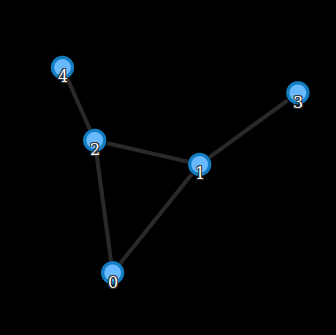
\includegraphics[scale=0.5]{bull.png}
\caption{Example Graph G=(V,E) Bull Graph (Created using the project)}
\end{figure}

The neighbourhood of a node or vertex $v_i$ is the set of
nodes $v_i$ is connected to, N($v_i$) = $\{v_j | (v_i, v_j) \in E, v_i \neq
v_j, 1 \leq j \leq n\}$. The degree of a node $v_i$, or the size of
the neighbourhood connected to $v_i$, is denoted as d($v_i$) =
$|N(v_i)|$. 
\par A degree sequence, \textit{D}, specifies the set of all node
degrees as tuples, such that D = {($v_i, d(v_i)$} and follows a
probability distribution called the \textit{degree distribution} with
mean $d_m$ \cite{githubtest1}.

\section{Graph Matrix Notation}
The matrix is commonly use dot represent grpahs for computer processing. The advantage of using matrix is usually that matrix algebra can be readily applied to study the structural property of matrix. There are number of ways in which one can represent the graph in it's matrix form for example, adjacency matrix and Laplacian matrix. 
\\
Let \textit{G}=(\textit{V},\textit{E}) be a simple graph with vertex set \textbf{V} and edge set \textbf{E}, then the adjacency matrix is square $|V|^2$ matrix \textbf{M} such that its element $M_{i,j}$ is \textit{1} when there is an edge from $v_i$ to $v_j$,where $v_i \in \textbf{V}$ , $ v_j \in \textbf{V}$ and \textit{0} when there is no edge.
The adjacency matrix of a graph of order \textit{n} entitles the entire the topology of a graph.  The diagonal elements of the adjacency matrix are all \textit{0} for undirected graphs \textbf{M}.

\par The sum of the elements of \textit{i}-th row or column yields the degree of node \textit{i}. If the edges are weighted, one defines the weight matrix \textbf{W}, whose element \textit{W}$_{ij}$ expresses the weight of the edges between vertices \textit{i} and \textit{j}.

\par The \textit{spectrum} of a graph \textbf{G} is the set of eigenvalues of it's adjacency matrix \textbf{M}. If \textbf{D}  is the diagonal matrix whose element \textit{D}$_{i,i}$ equals its degree of vertex $i$ ($v_i \in$ \textit{V}) \cite{matrep}.

\section{Approaches}
In this section we discuss the various approaches that are involved in dealing with the input to the project for community identification, for clustering and for visualization purposes. 
\subsection{For Community Identification}
Virtually in every scientific field dealing with empirical data, primary approach to get a first impression on the data is by trying to identify groups having "similar" behaviour in data. There are numerous methods to achieve this objective of which 

\begin{itemize}
\item Community Detection
\item Clustering
\end{itemize}

\subsubsection{Community Detection}
\subsubsection{Definition of a Community}
Communities are a part of the graph that has fewer ties with the rest of the system. Community detection traditionally focuses on the graph structugmres while clustering algorithms focuses on node attributes. 

Several tyoes of community detection algorithms can be distinguished
\paragraph{Divisive algorithms}
Divisive algorithms detect inter-community links and remove them from the network

\paragraph{Agglomerative algorithms}
Agglomerative algorithm merges similar nodes or communities in a recursive manner.

\paragraph{Optimization Methods}
Optimization methods are mainly based on maximization of an objective function.




\subsubsection{Clustering}
According to the paper "Community detection in graph" \cite{communitypaper} there are 4 major traditional clustering methods namely : 
\begin{itemize}

\item Graph Partitioning 

\item Hierarchical Clustering

\item Partitional Clustering

\item Spectral Clustering

\end{itemize}

\paragraph{Graph Partitioning}
This problem deals with dividing graph into groups of predefined size such that the number of edges between the groups is minimized. The paper \cite{communitypaper}  also defines cut size as the number of edges lying between the clusters.  Figure ~\ref{grapar} shows a problem with 14 vetices and presents a solution for spliting into 2 groups. 
\begin{figure}[H]
\centering
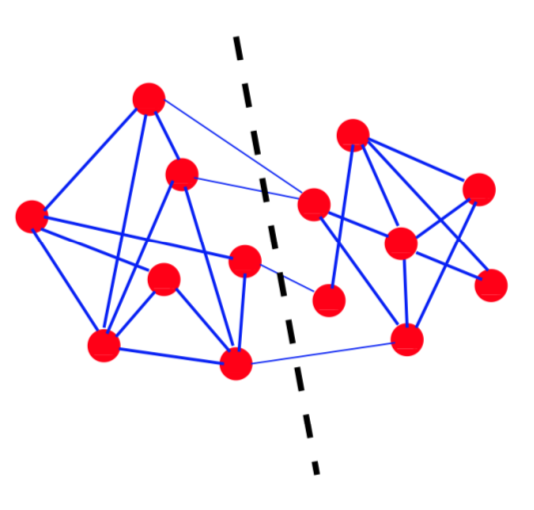
\includegraphics[scale=0.3]{graphpart.png}
\caption{\label{grapar}Graph Paritioning \cite{communitypaper}}

\end{figure}
\par \textit{Minimum Bisection Problem}, is a special problem case that considers partitioning the network into 2 groups of equal size. This problem is an NP-Hard problem. Intutively, to obtain ful partitioning we need to iteratively find all the minimum partition. This is not of significant use in the current problem of finding communities. 
\paragraph{Hierarchical Clustering}
Hierarchical clustering aims to identify groups of vertices with high similarities. It can be calssifies into two categories:
 \begin{enumerate}
\item \textit{Agglomerative algorithm} : in one in which Agglomerative algorithms, in which clusters are iteratively merged if their similarity is sufficiently
high
\item \textit{Divisive algorithms}, in which clusters are iteratively
split by removing edges connecting vertices with
low similarity.
The figure ~\ref{herar} demonstrates the hierarchcal clustering in a diagramatic manner.
\end{enumerate} 

\begin{figure}[H]
\centering
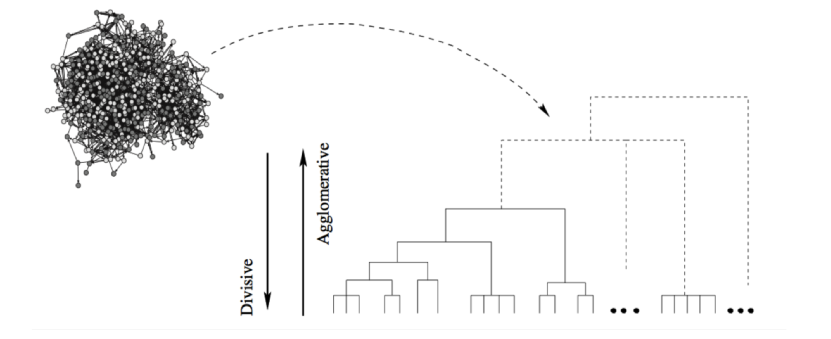
\includegraphics[scale=0.5]{hirac.png}
\caption{\label{herar}From a thickly knit graph to a dendogram [This intuitive diagram was taken from a powerpoint presentation for a data mining class]}
\end{figure}
\paragraph{Partitional Clustering}
Partitional clustering is method to find the clusters as a set of data points.  The number of clusters is preassigned. let us call this number as $k$. The vertex is a point on the metric space with a defined distance measure between the pair of points in the space.  The distance represents the difference in dissimilarity between the vertices. The main objective in this method is to separate the points in $k$ clusters such to maximize ((or) minimize) a given cost function based on distances between points and from points to $centroids$ that are suitably defined positions in space. 
Some of the most used functions are : \textit{Minimum k-clustering} ,  \textit{k-clustering sum}, \textit{k-center} and \textit{k-median}. One of the most popular partitional technique in literature is \textit{k-means clustering} where the cost function is total intra-cluster distance \cite{communitypaper}. This method of clustering is out of scope for the project in concern.
\paragraph{Spectral Clustering}
According to the paper \cite{communitypaper}, Let us suppose to have a set of $n$ objects $x_1 , x_2 , \ldots , x_n$
with a pairwise similarity function S defined between
them, which is symmetric and non-negative (i. e.,
S($x_i , x_j$) = S($x_j , x_i$) $\geq$ 0, $\forall$i,j = $1, ..n$). Spectral clustering includes all methods and techniques that partition
the set into clusters by using the eigenvectors of matrices,
like S itself or other matrices derived from it. In particular, the objects could be points in some metric space,
or the vertices of a graph. Spectral clustering consists of
a transformation of the initial set of objects into a set of
points in space, whose coordinates are elements of eigenvectors: the set of points is then clustered via standard
techniques, like \textit{k-means clustering}.

\subsection{For  Visualization}
Graph visualization is a important task in various scientific application. Visualization of data as graphs Visualizing these data
as graphs provides the non-experts with an intuitive means
to explore the content of the data, identify interesting patterns,
etc. Such operations require interactive visualizations
(as opposed to a static image) in which graph elements are
rendered as distinct visual objects; e.g., DOM objects in a
web browser. This way, the user can manipulate the graph
directly from the UI, e.g., click on a node or an edge to
get additional information (metadata), highlight parts of the
graph, etc. Given that graphs in many real-world scenarios
are huge, the aforementioned visualizations pose significant
technical challenges from a data management perspective \cite{graphviz}.

\section{Computational Complexity}
 The estimate of the amount of resources required for by the algorithm to perform a task is defined as computational complexity. The humongous amount of data on the real graphs or real networks that are available in the current scenario causes the efficiency of the clustering algorithm to be crucial.
\par In a brief, Algorithms that have polynomial complexity describe the Class \textbf{P}. Problems whose solutions can be verified in a polynomial time span the class \textbf{NP} of \textit{non--deterministic polynomial time} problems, which includes \textbf{P}. problem is \textbf{NP}-hard if a solution for it can be
translated into a solution for any \textbf{NP}-problem. However,
a \textbf{NP}-hard problem needs not be in the class \textbf{NP}. If it
does belong to \textbf{NP} it is called \textbf{NP}-complete. The class
of \textbf{NP}-complete problems has drawn a special attention
in computer science, as it includes many famous problems like the Travelling Salesman, Boolean Satisfiability
(\textbf{SAT}), Integer Programming, etc.
The fact that \textbf{NP} problems have a solution which is verifiable in polynomial
time does not mean that NP problems have polynomial
complexity, i. e., that they are in \textbf{P}. In fact, the question of whether \textbf{NP}=\textbf{P} is the most important open problem in theoretical computer science. \textbf{NP}-hard problems
need not be in \textbf{NP} (in which case they would be \textbf{NP}-complete), but they are at least as hard as \textbf{NP}-complete
problems, so they are unlikely to have polynomial complexity, although a proof of that is still missing. Reference to this has been imbibed from the paper "Community detection in graphs" \cite{communitypaper}.
\par Many clustering Algorithms or problems related to clustering are \textbf{NP}-hard. This makes it irrelavant to use the exact algorithm, in which case we use an approximation algorithm. Approximation algorithm are methods that do not deliver the exact solution but an approximate solution but with an advantage of lower complexity. \cite{communitypaper}

\section{State-of-the-art in Community Detection}
Modularity is the objective function that is widely used both as a measure and as a optimizing method for partitioning community.
As said before there are various algorithms that can be used for community detection . In reference to the paper \cite{generalcommunity} discusses six different community detection algorithms namely: 
\begin{itemize}
\item Louvain Method
\item Le Martelot
\item Newman’s greedy algorithm (NGA)
\item Newman’s spectral algorithm with refinement
\item simulated annealing
\item extremal optimization
\end{itemize}
The following figure ~\ref{Fig1} the average normalized performance rank of each algorithm in terms of partitioning quality and speed. Taken from the paper that proposed Combo algorithm \cite{generalcommunity}. 
\begin{figure}[h]
\centering
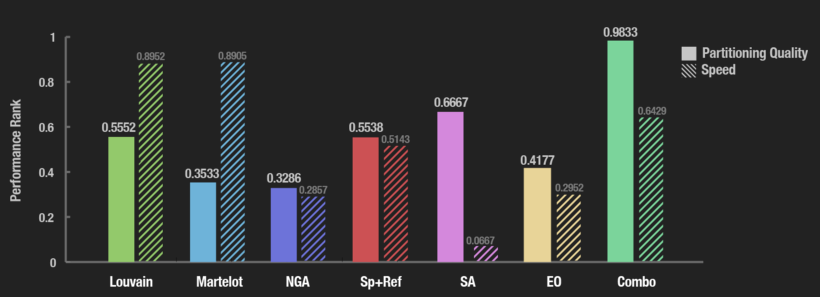
\includegraphics[scale=0.5]{lou.png}
\caption{\label{Fig1}Average normalized performance rank of each algorithm in terms of partitioning quality and speed}

\end{figure}
The main objective of the project is to visualize the data on screen thus needs an algorithm that is fast and should be effective.  Hence louvain algorithm was choose for the implementation. The implementation can be found in the later section of the report.


Louvain algorithm algorithm is considered as state-of-the art algorithm for community detection\cite{louvain}. The algorithm is fast,recursive and is more effective than the other algorithms in real-world graphs. Due to our goal of projecting medical domain we require an algorithm that gives a better trade off between being effective and being fast. Hence Louvain algorithm was chosen.

\section{Degree Distribution}
Degree of a node($v_i$) in the graph $G = (V,E)$ where $V$ is the set of vertices and $E$ is the set of edges is the number of edges that a  node has to other nodes. Usually denoted as deg($v_i$). \textit{Degree distribution} can be thus described as the probability distribution of there degrees over the entire graph.  Degree distribution is significant in the study of community networks and hence bringing it into consideration.  It is usually denoted as $P(k)$ of a graph which is the fraction of nodes in the network with degree $k$.
\begin{equation}
\begin{split}
P(k) &= \frac{N_k}{N}
\end{split}
\end{equation}
where $N_k$ is the number of  nodes with degree \textit{k} and \textit{N} is the total number of nodes in the graph.
\subsection{Scale-Free Graph}
The graphs whose degree distribution follows power law are called as Scale-Free graphs or scale free networks. 
\\
Examples of Scale-Free graphs include Social network graph,protein-protien interation network etc. 
According to the paper "Resilience of the Internet to Random Breakdowns" \cite{scalefree}, removing randomly any fraction of nodes from scale free network will not destroy the network which is in contract to Erdos-Renyi graphs. The figure ~\ref{ranfig} demonstrates how the random graph is different from a scale free graph.  The highlighted spots are knon as the hubs. For example: In a large community the celebrities or politicians serve as the hub. In scale free graphs another interesting feature is that as the clustering coefficient decreases with increase in the node degree. This type if distribution will be used in the experimental phase of the project for generating test cases. 

\begin{figure}[H]
\centering
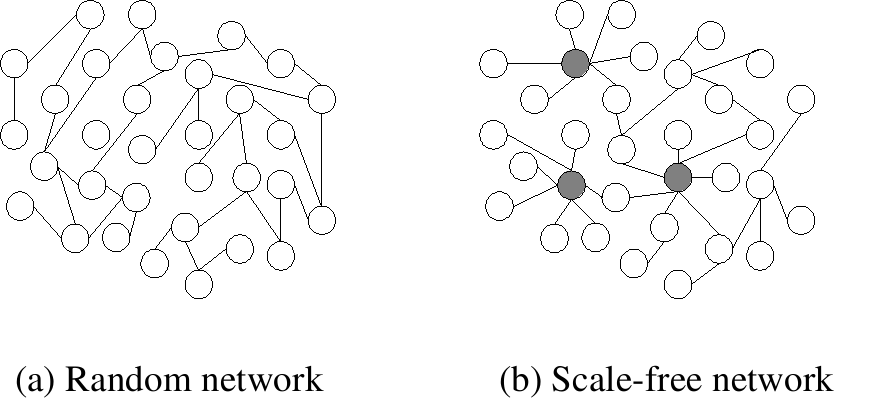
\includegraphics[scale=0.4]{sclaran.png}
\caption{ \label{ranfig} Random network (a) and scale-free network (b). In the scale-free network, the larger hubs are highlighted.(Image Source: Wikipedia)}
\end{figure}

\section{State-of-the-art in Graph Visualization}
Researchers have designed various tool-kits for the purpose of information visualization. Newer visualization techniques are introduced by creating new components or sub-classing the existing ones. The main aim of the project will be analyse the way inwhich the visual frameworks can be used and what kind of intermediate trasitions that are possible between the python program and the visualization framework. The project director's sugestion was to go with a JavaScript Library.

\textbf{Advantage of JavaScript Libraries} \cite{graphjslib}
\begin{enumerate}
\item \textit{Easy to use} : JavaScript is very easy to use, write and learn. It also saves time for the developer to write the code.
\item \textit{Reliable and standardized} : JavaScript libraries are more reliable and standardized and remains widely supported by several major web browsers. 
\item \textit{JSON is Standard}: JSON or JavaScript Object Notation is a standard input/output format for data sharing.
\item \textit{Simple and light-weight animation possible in JavaScript} JavaScript libraries need knowledge of CSS, HTML and editor to write the program. Contacting with Java or Adobe Flash , JavaScript animation require less learning and less time to make a cheap and effective animation 
\end{enumerate}

Due to these advantages JavaScript was suggested as the visualization as it is light, fast and data is easier to represent in JavaScript which satisfies the goal of the project. Next task is to find a JavaScript visualization framework.  

\par In the paper ``Effectiveness of JavaScript Graph Visualization Libraries in Visualizing Gene Regulatory Networks (GRN)" \cite{graphjslib} ``TABLE I" gives an summary of a few different JavaScript graph visualization libraries. Considering all the factor four of the visual techniques were chosen for the purpose of study and analysis of which one will be chosen for implementation. 
\subsection{Protovis}
Protovis is a domain-specific
language for constructing visualizations by composing simple
graphical marks such as bars, lines and labels. In Protovis, designers
specify visualizations as a hierarchy of marks with visual properties
defined as functions of data. Inheritance of properties across
composed marks similar to cascading of style sheets used in web
design enables concise visualization definitions with a large expressive
range and a minimum of intervening abstractions. Protovis is implemented
in JavaScript, with rendering support for HTML 5 canvas,
SVG, and Flash. The above extract is as given in the main paper about Protovis
\cite{protovis}.

\subsection{D3.js}
D3.js or simply D3 is a JavaScript library for manupulating documents based on data. D3 takes full advantage of cascading Style Sheets(CSS), HTML5 and Scalable vector graphics (SVG). D3 is viewed as the successor of Protovis. D3 targets at animation,interaction and complex and dynamic visualization in web.  It uses pre-built JavaScript
functions in its kernel in order to select elements, create SVG
objects, style them or add transitions and dynamic effects to
them.\cite{graphjslib}. Paper ``D3: Data-Driven Documents" \cite{d3} describes d3in its rightful way. D3 provides a wide set of example of which these were of great interest to the project:
\begin{enumerate}
\item
For graph: Force-Directed Graph, Labeled Force Layout,Forced Graph Editor , Directed Graph Editor, CodeFlower, University Program Transfers - Interactive, Better force layout node selection
\item For matrix visualization : Day/Hour Heatmap
\end{enumerate}
\subsection{Gephi}

Gephi is an open source software which use 3D render engine for visualization of graphs. 
A flexible and multi-task architecture brings new possibilities
to work with complex data sets and produce
valuable visual results. 
Gephi involves many key features in the context of interactive exploration and
interpretation of networks.  spatializing, filtering,
navigating, manipulating and clustering are allowed in Gephi.Dynamic network visualization is also possible in Gephi \cite{gephi}.
Although gephi is not JavaScript it is cited and considered for its externsive use in graph visualization. It is interesting to note that Gephi has JavaScript viewer such as JavaScript GEXF available on github. 

\subsection{Alchemy.js}
Alchemy.js is a JavaScript framework build entirely on d3. Goal of Alchemy.js is help the developer build and run graph visualizations with minimal overhead. A developer in Alchemy.js does not have to write much code to viaulize the data The very small amount of your work you do will actually just be in configuring Alchemy.js to visualize the data, along with whatever features you want to include in the application.

\chapter{Louvain Community Detection Algorithm}
In this section we describe the community detection algorithms such as Louvain and various tests that were performed to choose the algorithm. 
 
\section{Modularity}
The quality of partitioning that results from application of method is often measured using modularity. The \textit{modularity} of a partition is hence a scalar value between -1 and 1 that is used to measure the density of the links inside the communities as compared to the density of the links between the communities. This concept was first put forward by Newman \cite{newman2006modularity}.
\par
Modularity not only serves as a quality measure for detecting the quality of split or -partition, but also acts as an objective function to optimize.  Exact modularity optimization is \textbf{NP-Complete} in the strong sense \cite{modularityNP}.
\subsection{Definition}
Let G=(V,E) be a simple graph,where \textit{V} is the set of vertices and \textit{E} is the set of undirected edges. Let $n=|V|$ and $m=|E|$. Let degree of a vertex \textit{v} be, deg(\textit{v}) where \textit{v} $\in$ V. Let C be the community, $C \subseteq V$, be the subset of vertices. A \textit{clustering} $C_s =\{C_1,C_2, \ldots, C_k\}$ of G is a partition of V such each vertex is present exactly in one cluster.  We thus define \textit{modularity } as follows: \cite{modularityNP}

\begin{equation} \label{eq1}
\begin{split}
Q(C_s) &= \sum_{C \in C_s}\left[ \frac{|E(C)|}{m} - \left( \frac{|E(C)+\sum_{k \in C_s}|E(C,k)|}{2m} \right)^2 \right]
\end{split}
\end{equation}
where E(I,J) is set of all edges between vertices in cluster I and J. E(C) = E(C,C).
The above equation can be continently rewritten as follows: 
\begin{equation} \label{eq1}
\begin{split}
Q(C_s) &= \sum_{C \in C_s}\left[ \frac{|E(C)|}{m} - \left( \frac{\sum_{v \in C}deg(v)}{2m} \right)^2 \right]
\end{split}
\end{equation}
In simpler terms the value is of Q can be expressed as 
\begin{equation} \label{eq1}
\begin{split}
Q &= \left( \text{Number of Intra-Cluster Communities} \right) - (\text{Expected number of Edges})
\end{split}
\end{equation}

As given in \cite{louvain}

\begin{equation}
    \begin{split}
Q &= \frac{1}{2m} \sum_{ij} \left(A_{ij} - P_{ij}\right) \delta(C_i,C_j)
\end{split}
    \end{equation}

\begin{equation}
\begin{split}
\delta(C_i,C_j) &= \begin{cases} 1 ,& if C_i = C_j \\
 0,& otherwise
 \end{cases}
\end{split}
\end{equation}

where, $P_{ij}$ is the expected number of edges between nodes $v_i$ and $v_j$. $P_ij$ is $\frac{k_ik_j}{2m}$ where $k_x$ is sum of the weights of the edges attached to the vertex $v_x$ for a given random graph G (This is otherwise called as a null model).
    
\subsection{Properties of Modularity}
\begin{enumerate}
 \item Q depends on nodes in the same clusters only. 
  \item Larger modularity implies better Communities.
    \item 
    \begin{equation}
    \begin{split}
Q(C_s) \leq \frac{1}{2m} \sum_{ij} A_{ij} \delta(C_i,C_j) \leq \frac{1}{2m} \sum_{ij} A_{ij} \leq 1
\end{split}
    \end{equation}
 \item Value taken by Q can be negative
 \end{enumerate}
 
\section{Implementation of the Louvain Community detection Algorithm}
 Louvain algorithm is considered as the state-of-the art algorithm for community detection for identifying community structures \cite{louvain}. Louvain method developped by Blondel \textit{et al} \cite{louvain} finds high modularity partitions of large networks in short time. It unfolds a complete hierarchy community detection. 
 

\par

  The implementation is done using basic python packages. 
 The Algorithm has two phases that are repeated iteratively to bring the final solution to the problem. The following figure ~\ref{loupic} visualizes the steps in the algorithm and 
 Algorithm 1 defines a pseudocode for the Louvain method. 
\begin{algorithm}[H]
\caption{Louvain Algorithm Pseudocode}
\begin{algorithmic} 
\REQUIRE A graph G = (V,E)
\ENSURE Local optimum community split has happened

\WHILE{$Local Optimum Reached$}
\STATE Phase1 : Split or partition the graph by optimizing modularity greedily
\STATE Phase2 : Agglomerate the found clusters into new nodes
\ENDWHILE
\end{algorithmic}
\end{algorithm}


 \begin{figure}[h]

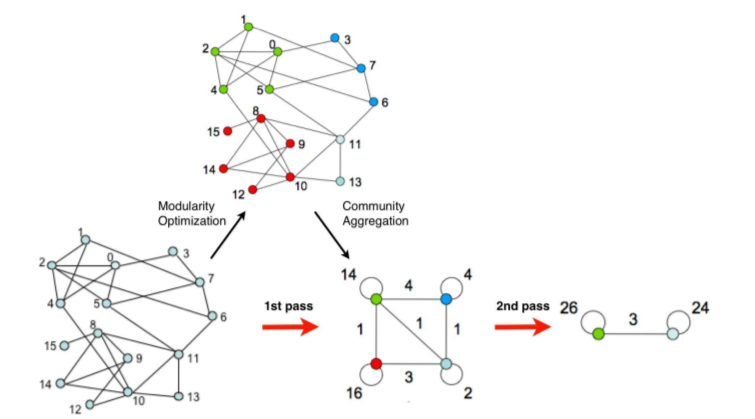
\includegraphics[scale=0.5]{loustep.png}
\caption{\label{loupic} Visualization of the steps of our algorithm. Each pass is made of two phases:
one where modularity is optimized by allowing only local changes of communities;
one where the found communities are aggregated in order to build a new network of
communities. The passes are repeated iteratively until no increase of modularity is
possible. This was taken from the paper "Fast unfolding of communities in large networks" \cite{louvain}}
\centering
\end{figure}

\subsection{First Phase : Optimizing Modularity}
In the first phase the algorithm assigns a different community to each node in the network.  The number of nodes is equal to the number of communities in the graph. Let $v_i$ be be a node such that $v_j$ $\in$ N($v_i$). The gain of modularity is then calculated by removing $v_i$ and placing it in community of $v_j$. If the gain is positive the $v_i$ is moved to the community of $v_j$ else $v_i$ stays in it's original community. This procedure is iterated and the phase one stops when a local maxima of the modularity is achieved, that is when no more move of nodes from one community to another is possible. The ordering of the nodes can affect or effect the computation time which can be a part of future works. 

\begin{algorithm}[H]
\caption{Phase 1 in Louvain Algorithm Pseudocode}
\begin{algorithmic} 
\REQUIRE A graph G = (V,E)
\ENSURE Partition network greedily using modularity
\STATE Assign a different community to each node
\WHILE{$Local Optimum Reached$}
\FORALL{Each node $v_i$}
\STATE{ For each node $v_j$ $\in$ N($v_i$), consider removing $v_i$ from community of $v_i$ and place it in the community of $v_j$}
\STATE Calculate the modularity gain
\IF {\textit{ModularityGain} is Positive}
\STATE remove $v_i$ from community of $v_i$ and place it in the community of $v_j$
\ELSE 
\STATE No Change
\ENDIF
\ENDFOR
\ENDWHILE
\end{algorithmic}
\end{algorithm}

\par The main algorithm relies on the calculation of modularity. Listing 3.1 demonstrated the calculation using a python snippet. The first phase of the algorithm has been written into a python code snippet and is presented in the Listing 3.2. 
In the paper it is stated that the gain in modularity as $\bigtriangleup$Q

\begin{equation}
\begin{split}
\bigtriangleup Q &= \left[ \frac{\sum_{in} + k_{i,in}}{2m} - \left( \frac{\sum_{tot} + k_{i}}{2m} \right)^2 \right] - \left[ \frac{\sum_{in}}{2m} - \left( \frac{\sum_{tot}}{2m} \right)^2 - \left( \frac{k_i}{2m} \right)^2 \right]
\end{split}
\end{equation}
where $\sum_{in}$ is the sum of the weights of the links inside C and $\sum_{tot}$ is the sum of the weights of the links incident to nodes in C, $k_i$ is the sum of weights of the links incident to node i, $k_{i,in}$ is the sum of the weights  of all the links in the network.

\subsection{Second Phase : Agglomerating the communities found in first phase into new nodes}
In the second phase the algorithm builds the new network. The communities that are found during the first phase are now the nodes here. According to the paper \cite{louvain}, the weights of the links between the new nodes are given by the sum of the weight of the links between nodes in the corresponding two communities. The edges between nodes of the same community lead to seld-loops for this community in the new network. The resulting new weighted network is then subjected to first phase  and this process is iteratively done. 
\begin{algorithm}[H]

\caption{Phase 2 in Louvain Algorithm Pseudocode}
\begin{algorithmic} 
\REQUIRE A graph G = (V,E)
\ENSURE Agglomeration of nodes
\STATE Every community $C_i$ forms a new node $v_i$
\STATE $W_{ij}$ = $\sum$ \{All edges between $C_i$ and $C_j$\} where $W_{ij}$ is the edge between newly formed nodes $v_i$ and $v_j$
\end{algorithmic}
\end{algorithm}
\section{Observations of Louvain}
\begin{enumerate}
\item The final output of the Louvain algorithm forms a complete hierachical structure.
\item Resolution limit problem \cite{ResolLimit} has been resolved in the algorithm stated in the current paper under discussion \cite{louvain} due to the multi-level nature of Louvain algorithm.
\item Modularity can be redefined for weighted graphs and Louvain works well with weighted graphs.
\end{enumerate}

\section{Mode of implementation of the Louvain Algorithm}
In the project the above algorithm has been implemented in python taking inspiration and reusing some part of the pylouvain program API for implementation \cite{pylouvain}. Using python was a requirement of the project directors, in case the code has to be reused in a larger ongoing project which is programmed in Python and Javascript. Hence Python was used to implement the Louvain Algorithm.

\section{Experiments}
In performing experiments we analyse the speed and capability of the python program to handle more input and also to see pattern of behaviour of the data. For this purpose test case inputs have to be generated or test cases that are available online must be used. 
In this project we utilize both method to see the performance of the program. All the tests were run on 2.50GHz Intel Core i5-3210M with 8 GB RAM (Sony Vaio) running gnome-ubuntu 14.04 operating system. 

\subsection{Nodes vs Time keeping modularity constant}
\par In the paper "Exploring community structure in biological networks with random graphs" \cite{githubtest1}, have developed a generative model to produce undirected connected graphs with a degree and a pattern of communities while maintaining a graph strucuture that is as random as possible.  They have given 2 programs one which contains the degree distribution funtions such as scale-free degree  distribution, poisson degree distribution, regular distribution and geometric.  In this project we are intersted in scale-free distribution as most real-world networks are scale free in nature \cite{scalefree}. To run this test networkx package is a necessary component. 

\par For the purpose of testing 2 programs in python were written. First program is a generator program that sets the degree distribution to scale-free, Q=0.4 [ Average Q value ] and N=150 to N=2300. This porgram generate a set of files conatins graphs with nodes in the range of N. Second program is the ploting program in which the files that were generated in the first program was supplied as input to the second program and Louvain algorithm was applied. Time of run for Louvain was calculated for each input and recorded. This was then ploted into graphs using the matplotlib function. The graphs are displayed in figure ~\ref{ex1}, ~\ref{ex2}, ~\ref{ex3} and ~\ref{ex4} for respective range of nodes mentioned in the caption of the graphs.

\begin{figure}[H]
\centering
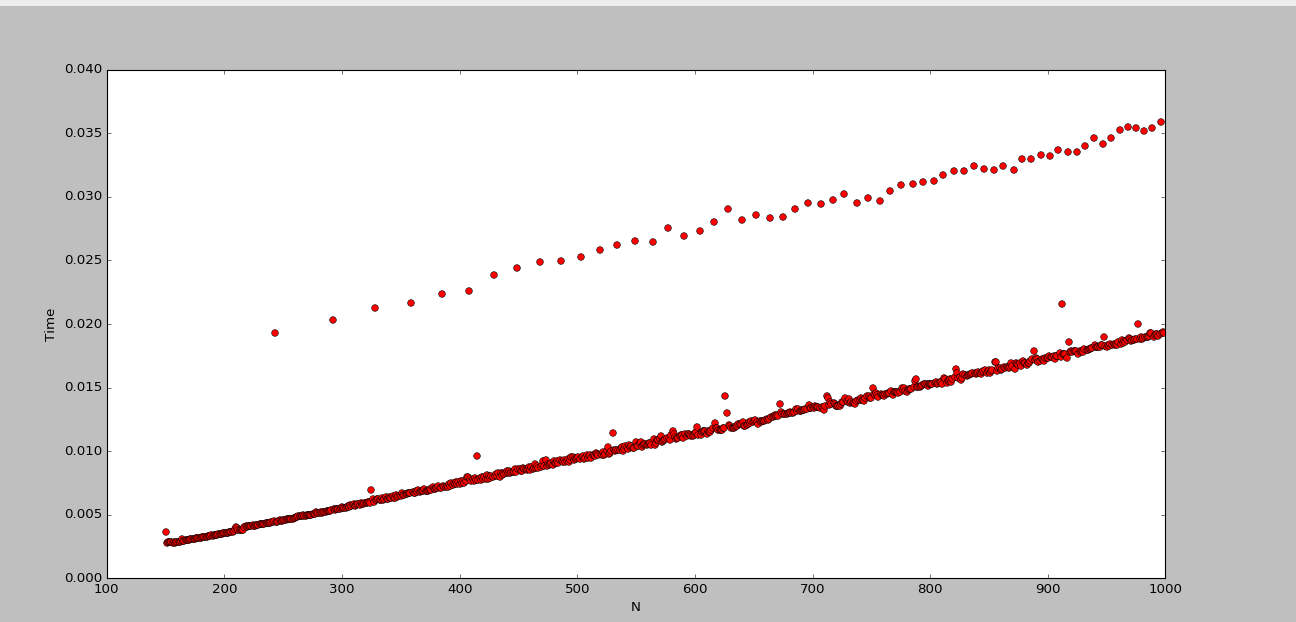
\includegraphics[scale=0.3]{e1000.png}
\caption{\label{ex1}Experiment showing the plot of time vs number of nodes for 1000 nodes}
\end{figure}

\begin{figure}[H]
\centering
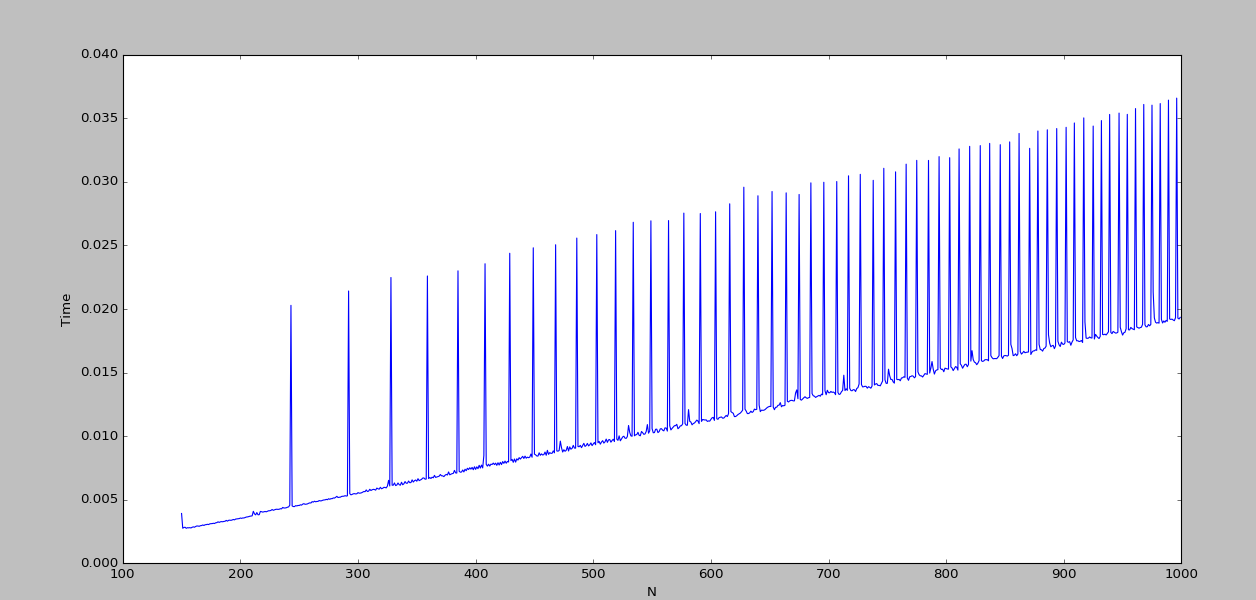
\includegraphics[scale=0.3]{e1000b.png}
\caption{\label{ex2}Experiment showing the plot of time vs number of nodes for 1000 nodes points joint by lines}
\end{figure}

\begin{figure}[H]
\centering
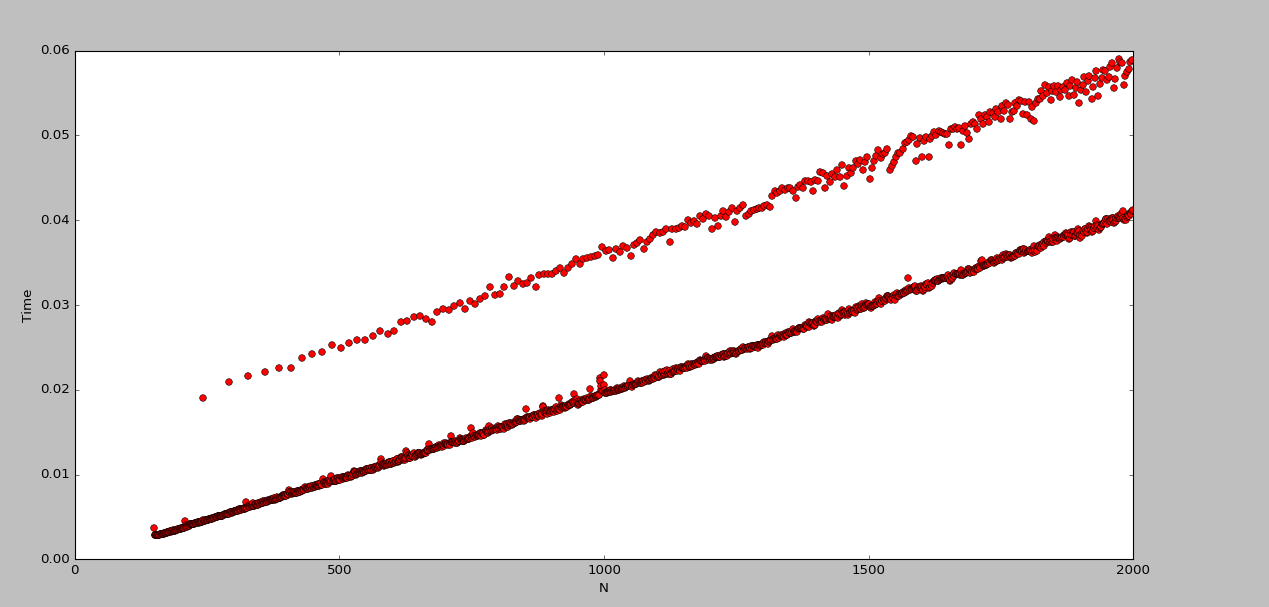
\includegraphics[scale=0.3]{e2000.png}
\caption{\label{ex3}Experiment showing the plot of time vs number of nodes for 2000 nodes}
\end{figure}

\begin{figure}[H]
\centering
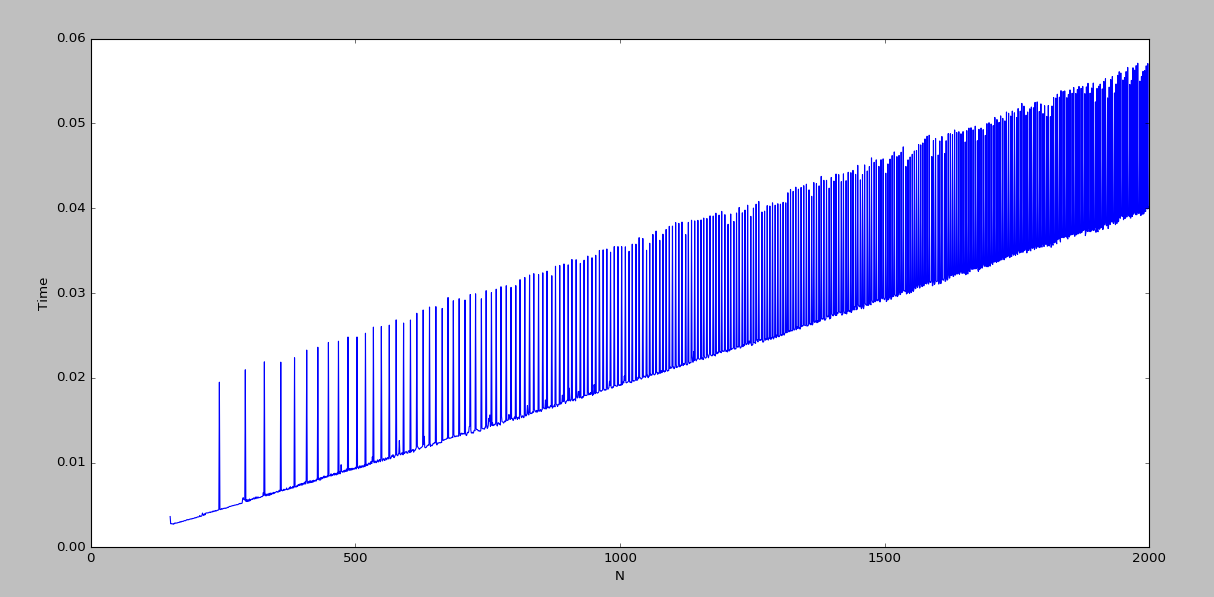
\includegraphics[scale=0.3]{e2000b.png}
\caption{\label{ex4}Experiment showing the plot of time vs number of nodes for 2000 nodes points joint by lines}
\end{figure}

\par It  is interesting to note that for steady raise in the number of inputs there was a steady raise in the time. There were very few jitters that were caused by the computer.

\subsubsection{Minor bugs}
In the results obtained it is intersting to note that there is a set of slow runs that occur at regular intervals. These are due to the effect of garbage collection done by python automatic garbage collector. This issue was found by manually turning of the garbage collection and explicitly calling it every time after each run. 

\subsection{SNAP}

A collection of more than 50 large network datasets from tens of thousands of nodes and edges to tens of millions of nodes and edges. In includes social networks, web graphs, road networks, internet networks, citation networks, collaboration networks, and communication networks.
\cite{snap}
\begin{figure}[H]
\centering
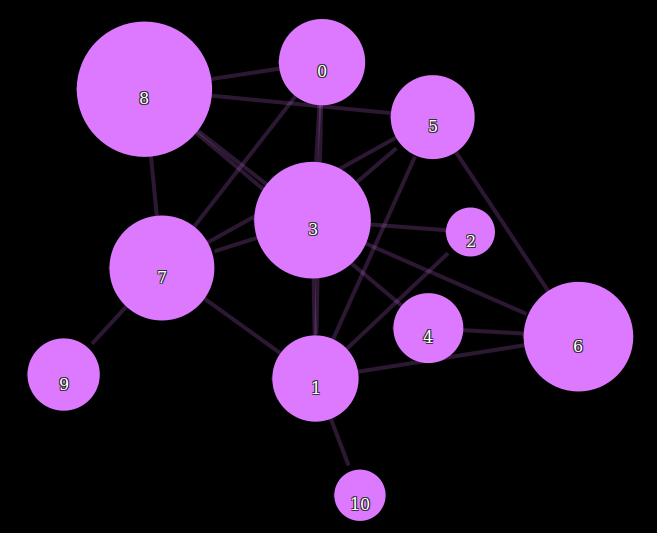
\includegraphics[scale=0.3]{fb.png}
\caption{Example Graph G=(V,E) Bull Graph}
\end{figure}

\subsection{igraph tests}
Python provides an exciting package on igraph. igraph 
\cite{igraph}

\section{Result}

\chapter{Visualization Module}
Visualization module is developed keeping in mind that python API must exist and should be JavaScript based.As already said these were the requirements that were set by the project directors. In this section an analysis of the selected software and method of choice by exploring all the possible ways will be explained. 
\section{Exploring the state-of-the-art}
For visual representation, softwares such as Protovis, D3, Alchemy.js and Gephi were tested
using example graphs.  Gephi is a tool
used for data analysis for understanding and exploring graph based data,however it has some
drawbacks in the logistics of the project such as Gephi is not JavaScript based although it has a JavaScript viewer. Gephi has more overhead being a software than a simple framework. For a similar reason we refrain from using softwares such as HyperTree, HyperGraphs as they did not have a python API or are not based on JavaScipt but instead has a
Java Code based APIs.  D3
provided the necessary tools and was JavaScript and could be linked to python and was the best
option for the project's logistics. Alchemy.js was built using D3. Alchemy.js required minimal code
to generate the graphs as most of the customization could be done by just overriding or altering the
“config” [Configuration part of the Alchemy.js] instead of implementing it entirely using
JavaScript. Alchemy.js also provides a feature in which the core application can be further extended
with any other feature of D3. Having D3 to be the base, with minimal code and maximum
customization Alchemy.js was chosen for visual representation of the graph in this project. Protovis provides a matrix representation in the form of a matrix diagram.  Thus the project directors also considered alchemy.js as a visualization software as it fits the bigger project for graph visualization and Protovis API was used to visualize matrix representation. 


\section{Alchemy.js}

Alchemy.js is a graph drawing library built to provide graph visualization with little overhead. It is built on the d3 library, written in Javascript, which runs in most web browsers.   

\section{Dependencies for Alchemy.js}
Alchemy needs three main units to  form as an application namely:  \textit{alchemy.css}, \textit{alchemy.js} and \textit{data}. CSS and JavaScript are major dependencies in Alchemy.js. Installation of \textit{jQuery} and \textit{d3} is also useful. \textit{alchemy.min.js}, \textit{alchemy.css} and \textit{alchemy.min.css } will be updated in the CDN (Content Delivery netwrok)
\section{Steps to use the Alchemy.js}
 In this project we have uploaded the \textit{alchemy.min.js}, \textit{alchemy.css} and \textit{alchemy.min.css } into the project's file repository http://abhinavsv3.github.io/javascriptsal and hence will be using the link in the following explanation. 
The following describes the steps that are followed in use of Alchemy.js :
\begin{enumerate}

\item \textit{Include the files in this format}\\
$<$link rel="stylesheet" href="http://abhinavsv3.github.io/javascriptsal/alchemy.min.css"/$>$
\\
\ldots\\
$<$script src="http://abhinavsv3.github.io/javascriptsal/alchemy.min1.js"$></script>$

\item \textit{Include an element with "alchemy" ID as the id and class }\\
The alchemy class is used to apply styles while the alchemy id is used programatically. By default Alchemy.js looks for the alchemy div but this can be overridden.
$<$div class="alchemy" id="alchemy"$><$/div$>$

\item \textit{Provide Alchemy.js with a JSON dataSource}

\item \textit{Begin Alchemy.js}
$<$script$>$
  alchemy.begin$(\{"dataSource": someData\})$
$<$/script$>$



\end{enumerate}
\section{Protovis for Matrix Display}
Protovis is considered as the predecessor D3.js. In Protovis there is an example for Matrix Diagrams. This example is of keen interest for the project for representing the data.It is JavaScript and can be visualized with just the JavaScript matrix as input.
\par Since this is the only component that is taken from Protovis a Protovis template was adopted and from the Protovis repository and integrated with the project.

\section{Getting the data from the Louvain Python code to Alchemy. }
 Alchemy.js takes a simple data format called GraphJSON. GraphJSON serves as a light weight and flexible representation of graph data, easily consued locally or over the web. 
\par 
GraphJSON is a JSON Object which has 2 object namely: \textit{nodes} and  \textit{edges} . These are individual arrays that represent the nodes and edges that will be represented in the graph visualization. 
\par \textbf{Nodes} : id key is the only unique value that should be present in the nodes
\par \textbf{Edges} : source and target key are the only unique value that should be present in the edges.
\par A python program was implemented to convert the output of the louvain program into json object using the python json package. This converts the output of the louvain program into two JSON object. one JSON object 
This can be seen as the advantage of system. We compute once and reuse the computed result for various visualizations.
\par For the matrix representation the JavaScript file containing the matrix is created which is used by the protovis program to display and reorder the matrix.

\section{Tests}
For the purpose of visualization various test were performed for analysing the compatibility of Alchemy.js and to explore and exploit all the functionalities of alchemy.js and choose the best ones for the project and implement them.Protovis for the matrix visualization was used.
\subsection{Alchemy.js Tests}
The following will enumerate the tests that were performed one after another. Github pages were used to test host the web visualization.

\begin{enumerate}
\item Test1 and Test2
\par \textit{Test1} consists of providing the JSON object as input to the Alchemy.js to build a normal graph. Test 1 is performed to see if the nodes can be selected, viewed and seperated.
\par \textit{Test 2} Test2 uses the same JSON object as input.In Test2 the Test1 graph is presented with custom graph weight, graph width and link distances. This makes it easier to integrate it with larger application. Figure ~\ref{test1} shows the graph that was used to perform test1 and test2.

\begin{figure}[H]
\centering
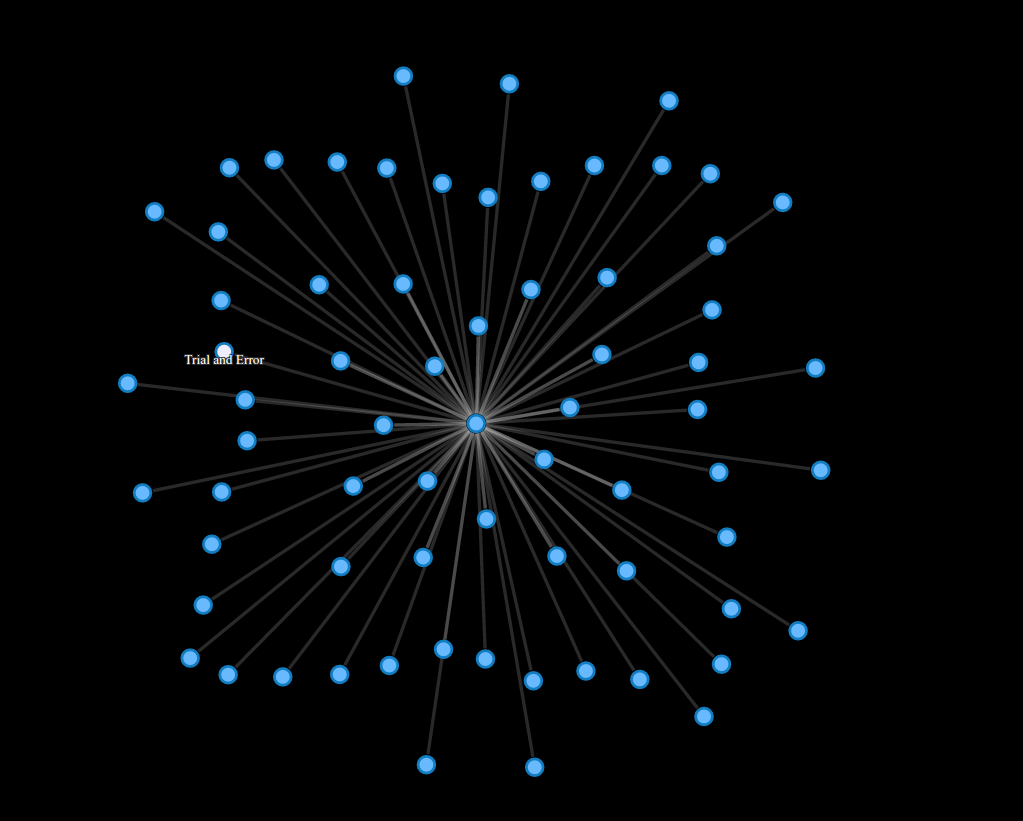
\includegraphics[scale=0.3]{t1.png}
\caption{\label{test1}Test 1 and Test 2 look the same. The JSON object has been taken from Alchemy.js Examples. One named node ``Trial and Error" has been selected and viewed.}
\end{figure}

\item \textit{Cluster Assignment Test}
\par In this test cluster assignment is tested.Clusters are assigned in the JSON object by setting values for the cluster in the form of cluster number and assign seperate colors for these clusters.	Thus, this test focussed on node clustering or node coloring to assign each node into its cluster. Figure ~\ref{test3} show the result of the test(Test3). 

\begin{figure}[H]
\centering
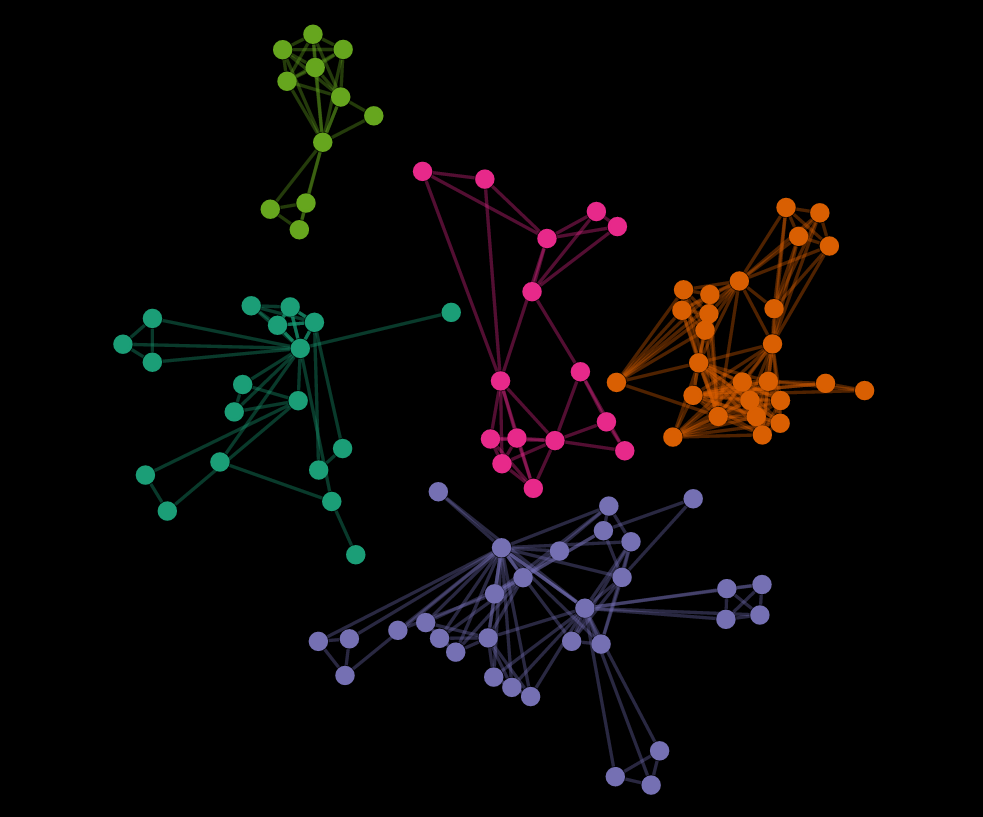
\includegraphics[scale=0.3]{t2.png}
\caption{\label{test3}Clustering based Alchemy.js.  The JSON object has been taken from Alchemy.js Examples.}
\end{figure}

\item \textit{Directed and weighted edges}
\par In this test we explore the special JSON object with directed and weighted edges. The test also shows an instance of controlling edge thinkness, node diameter and node thickness(Test4). Figure ~\ref{test4} shows an example of this test.
\begin{figure}[H]
\centering
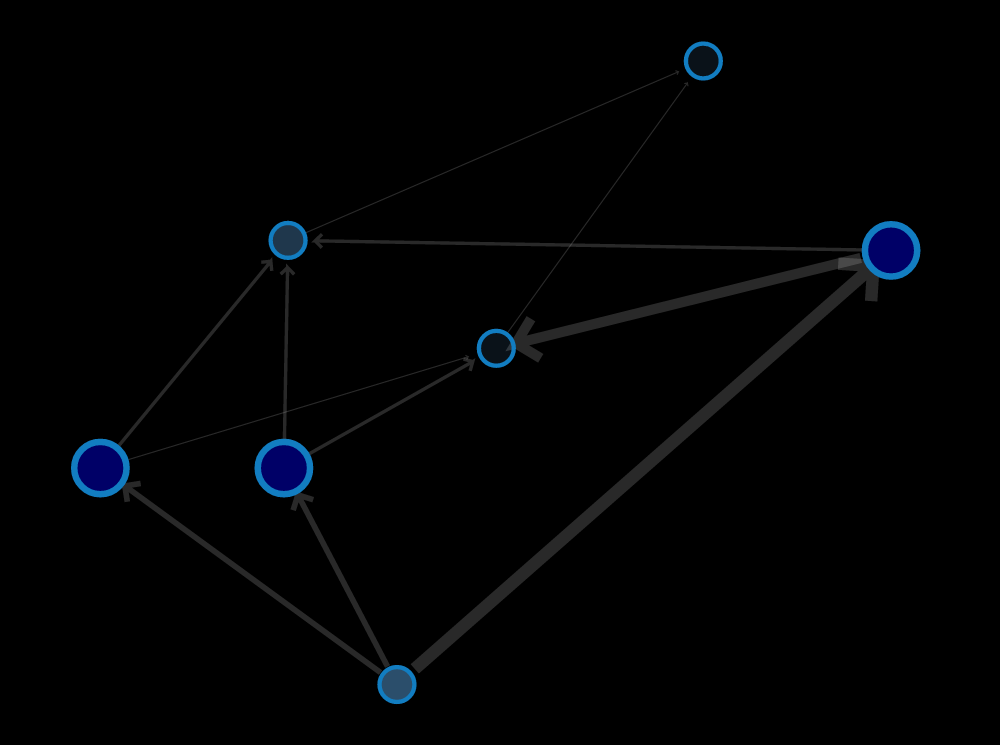
\includegraphics[scale=0.3]{t3.png}
\caption{\label{test4}Example Directed and weighted edges.  The JSON object has been taken from Alchemy.js Examples.}
\end{figure}

\item \textit{Network}
\par A test in which a hairball network is generated having roots and nodes.  Figure ~\ref{test5} shows an example of seven minutes of communication between members of the AngularJS, EmberJS, and KnockoutJS IRC channels(Test5).

\begin{figure}[H]
\centering
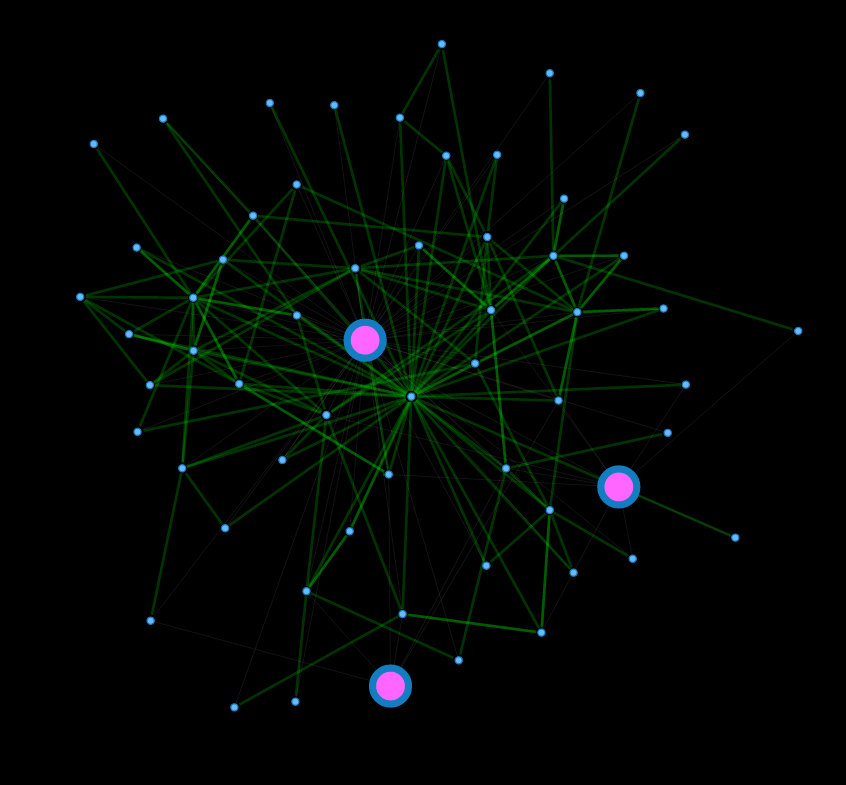
\includegraphics[scale=0.3]{t4.png}
\caption{\label{test5} Seven minutes of communication between members of the AngularJS, EmberJS, and KnockoutJS IRC channels. JSON object taken from the Alchemy.js examples.}
\end{figure}

\item \textit{Graph with relatedness}
\par A test in which a graph with relatedness was generated. Figure ~\ref{test6a} shows a sample having relatedness between philosophers. Figure ~\ref{test6b} shows a zoomed view of one of the philosopher graph (Test6).

\begin{figure}[H]
\centering
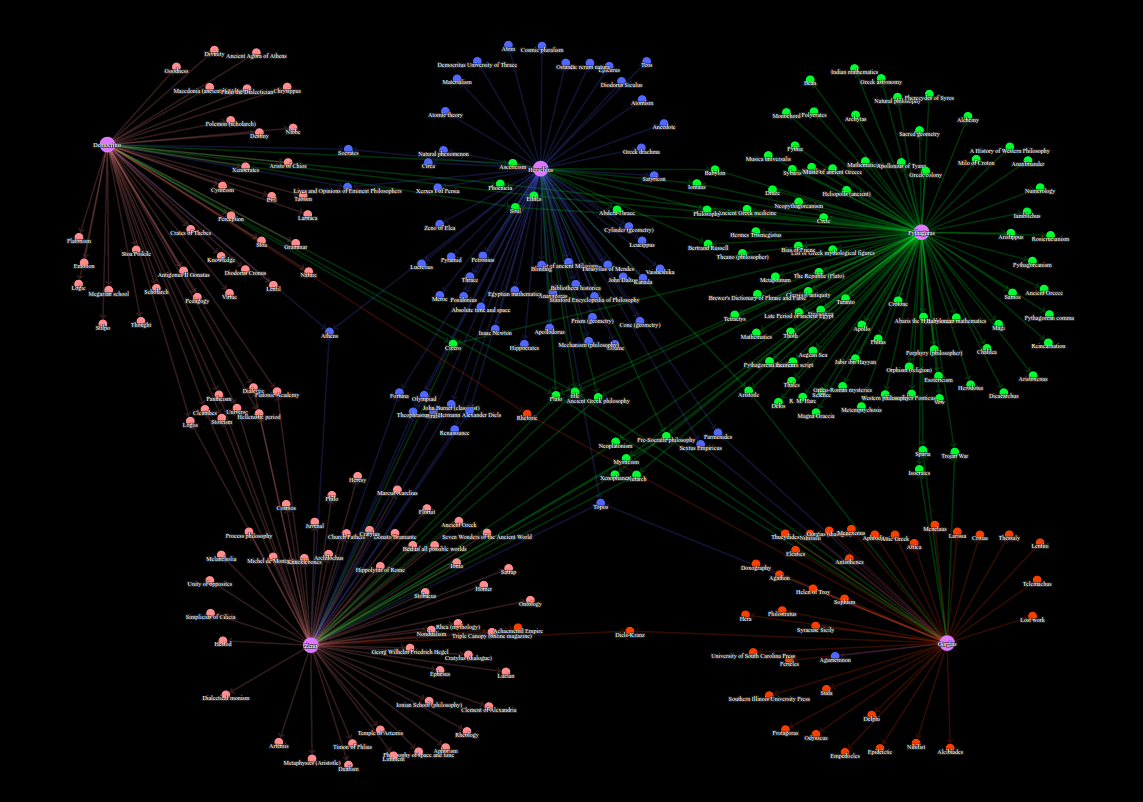
\includegraphics[scale=0.3]{t5.png}
\caption{\label{test6a}A graph in which the relatedness of scientists to the philosopher is shown. This example JSON was take from Alchemy.js example graphs}
\end{figure}

\begin{figure}[H]
\centering
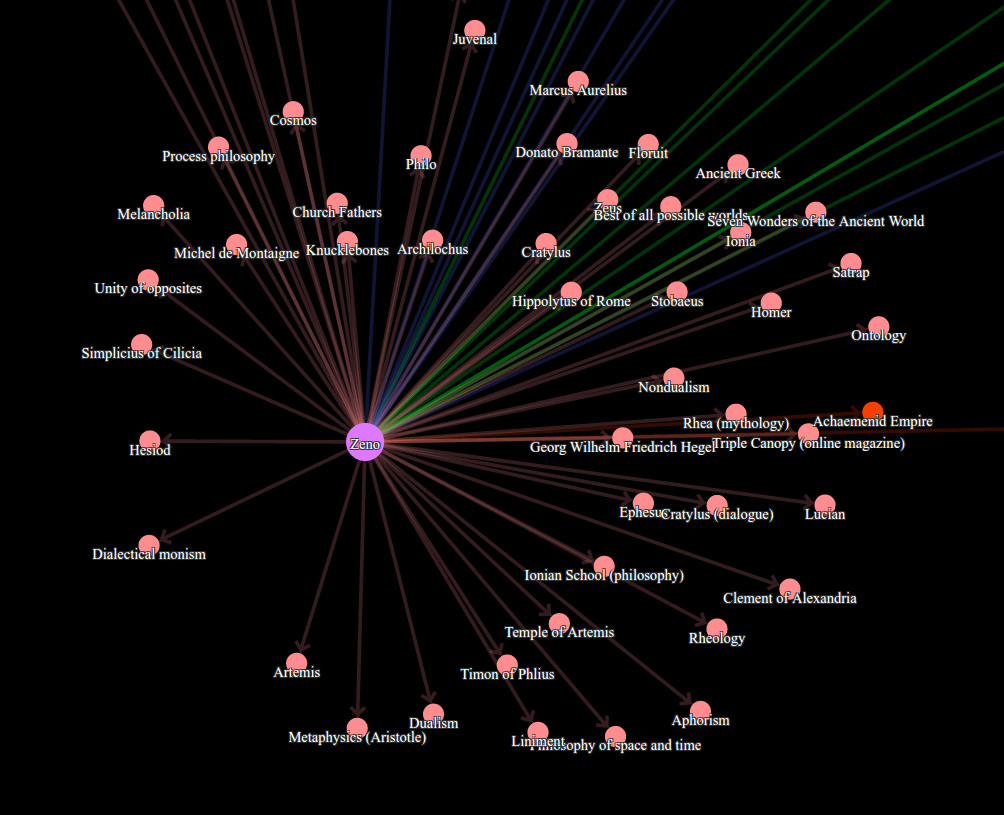
\includegraphics[scale=0.3]{t6.png}
\caption{\label{test6b}Closeup view of one of the philosopher.}
\end{figure}

\item \textit{Node Area and Color}
\par In this test the difference in node are and assignment of colors to nodes was tested. Figure ~\ref{test7} presents can example in which the test is performed (Test7).


\begin{figure}[H]
\centering
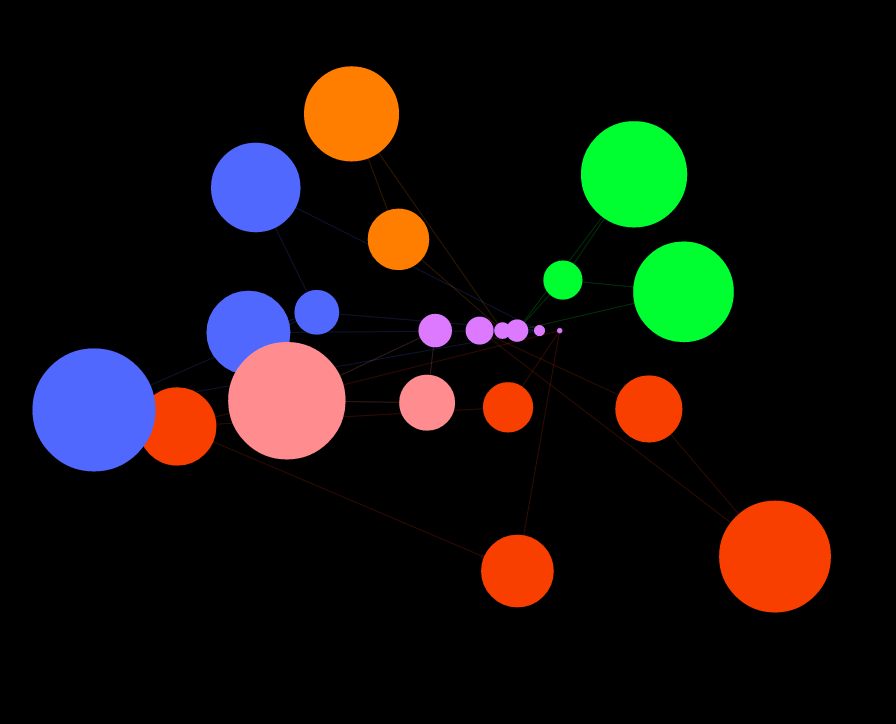
\includegraphics[scale=0.3]{t7.png}
\caption{\label{test7}Node area and node color.JSON object created manually.}
\end{figure}
\end{enumerate}

\par After performing all the test few of the desired features were incorporated to fordisplaying th graph in the project. The project uses test7 for showing the size or the bulkiness of the node in comparison with other node. Test6 relatedness has also been added to the project to mark the edge values between the nodes. Test3, clustering has also been added to the project.
\subsection{Protovis Tests}
For the purpose of matrix visualization, protovis has been implemented in the project. A test run of it is presented in the Figure ~\ref{test8}.
\begin{figure}[H]
\centering
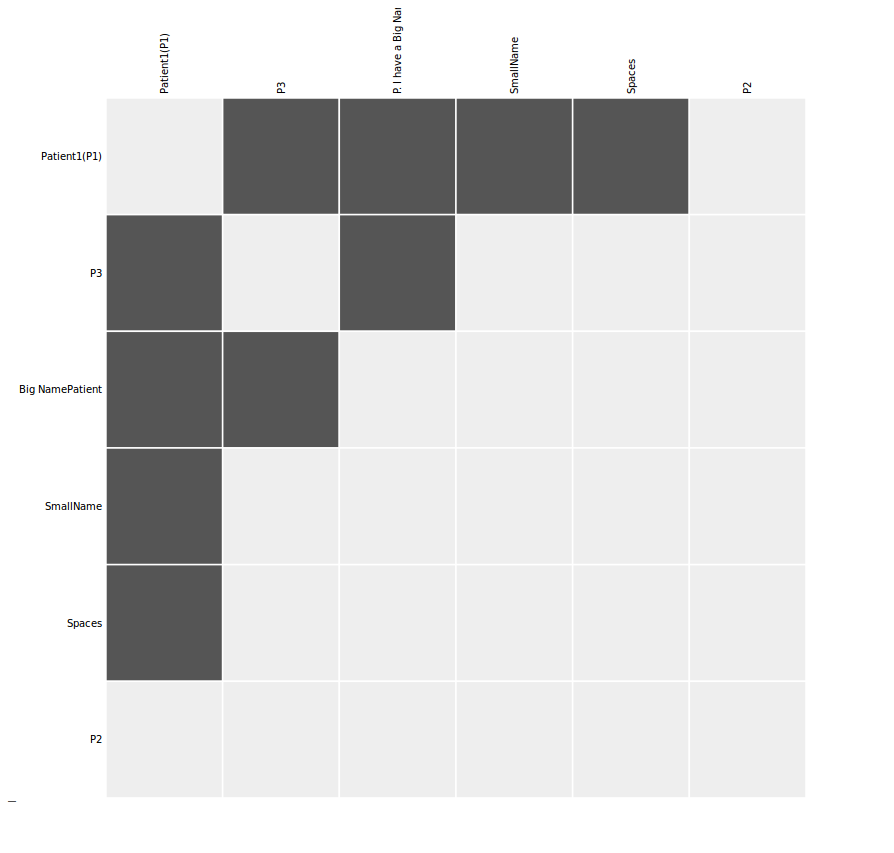
\includegraphics[scale=0.3]{d4b.png}
\caption{\label{test8}Matrix Visualization.}
\end{figure}


\subsection{Bug Report}
In the project there was minor issues that were to be addressed:
\begin{enumerate}
\item  Alchemy.js does not render a few
edges on screen when using web browsers that such as Google chrome. Mozilla Firefox use Gecko
which helps to read web contents like JavaScript, html, css etc better than in Google chrome. Thus,
it is recommended to run the project on mozilla firefox or sea monkey than on Google Chrome.
\item \textit{Bug Number 472}: It was found when rendering of edges is an bug that was reported in Alchemy.js issues as Bug number : 472 ( \url{https://github.com/GraphAlchemist/Alchemy/issues/472}). We have also reiterated the issue. The issue is that in the graph where the communities are rendered seperately wil colors the edges that run between two communities are names and weights are assigned but the edge is not rendered.
\end{enumerate}

\section{Result}
Finally the project adopted alchemy.js for the graph representation and Protovis layout for the matrix representation.  The errors were verified and necessary tests were performed to ensure that the visualization process runs smoothly. 

\chapter{Overall System Description}
The project uses two complementary technologies of a raw python code and a JavaScript program that can represent or draw the output of the python code on screen. This lead to a need to include a new element of a web framework for implementing the louvain algorithm and creating a JSON object, and JavaScript to represent the graph on a web browser.   A web framework is one that aims to remove the overhead associated with common activities performed in the web development. 
\section{Choice of Web.py}
An exploration one a few python web frameworks such as Django, Grok and web.py. A sample application in Django was built to see if Django suits the need of the project. Django was eliminated due to the fact that it was heavier for a simple task that we wish to perform in the project. Web.py was chosen as the web framework for the project as it allowed successful integration  of the existing python code with the web framework over grok.We must note that the larger project at the LARCA group does not use web.py instead another framework called Angular.js. However, Angular.js is designed to be used for large, complex projects, and after some evaluation it was clear that the overhead for this small project did not pay off. 
Thus, Web.py suffices and was easy to used for the current need of the project that is to perform the integration task.  

\section{Frontend Framework}
Bootstrap was an intuitive web front-end frame work that has been implemented in the project.  Bootstrap allows to divide the screen into various matrix cubes enabling us to place buttons to run the application. Bootstrap, originally named Twitter Blueprint, was developed by Mark Otto and Jacob Thornton at Twitter as a framework to encourage consistency across internal tools. It is the second most starred project in github and has more than forty thousand forks \cite{bootstrap}.


\section{Using the application}
The web application thus developed is intutive enough such that even though it performs tasks of computation and integration into the web it looks simple. Minimal and most necessary elements have been implemented.
In the following we describe the entire working flow of the Web Application:
\begin{enumerate}
\item \textbf{"Login Page"} In this part a simple login password is described.  
\begin{figure}[H]
\centering
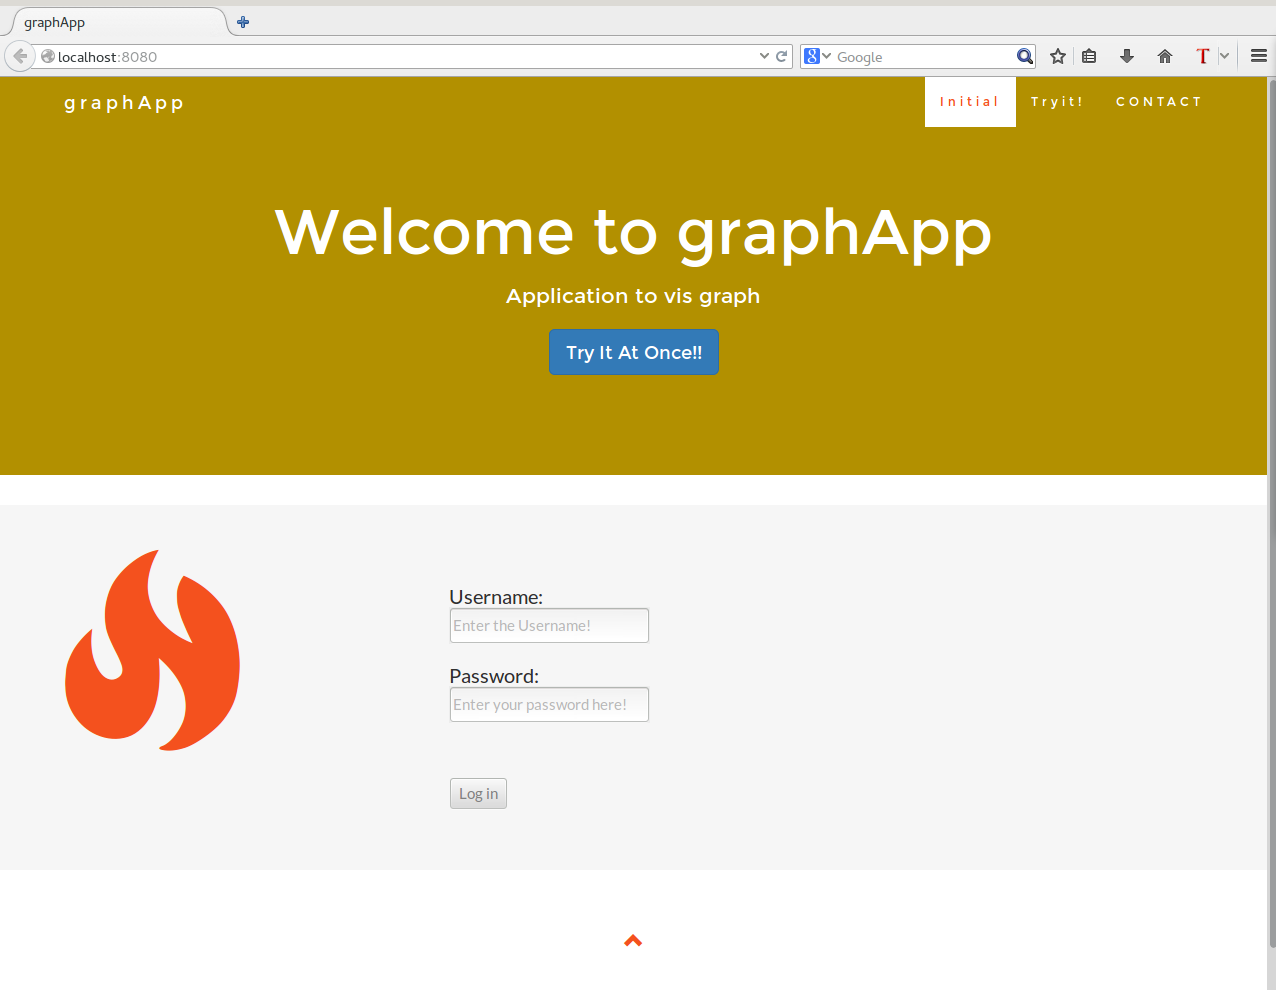
\includegraphics[scale=0.3]{s1.png}
\caption{Landing page containing login}
\end{figure}

\item \textbf{File Loader Page} After logining the user lands in a file loader page where provision has been provided to upload a text file containing the adjacency matrix of the graphs are present in the "start" "Destination" or "Start" "Weight" "Destination" format. In this space only numerical values can be accepted for supporting the simplicity of the background process. Another space to provide a key that maps the names of the node numbers. This helps to present another dimension of seeing the data in the form of names.  Viewing the names of the node over nodes helps the user to deepen his vision of analysis. 
\begin{figure}[H]
\centering
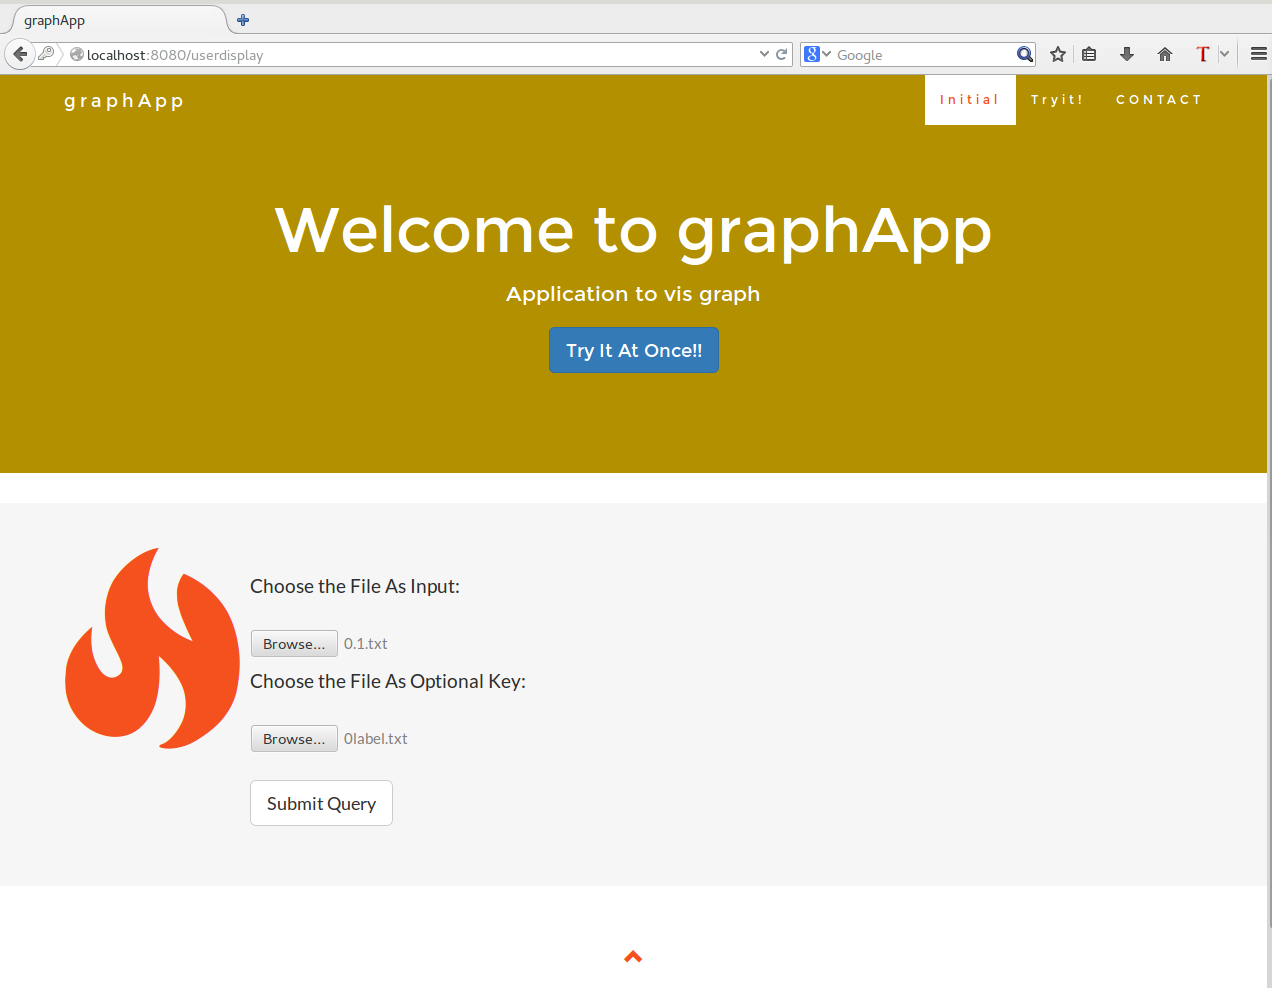
\includegraphics[scale=0.3]{s3.png}
\caption{After login, the application asks for the data and/or key }
\end{figure}


\item \textbf{Dash Board} In this part of the web application the user lands in a page that presents to the user 4 different variety of visual representation of the input data :  Community graphs (Diplaying the links between various communities), Full graph split into communities represented with different colors, Original graph input(Helps to see if the input was proper) and a Matrix view of the graph

\item \textbf{On Click Viz.} On clicking on the visualization the user wants to take the web aplication switches to the graph that the user has clicked.

\begin{figure}[H]
\centering
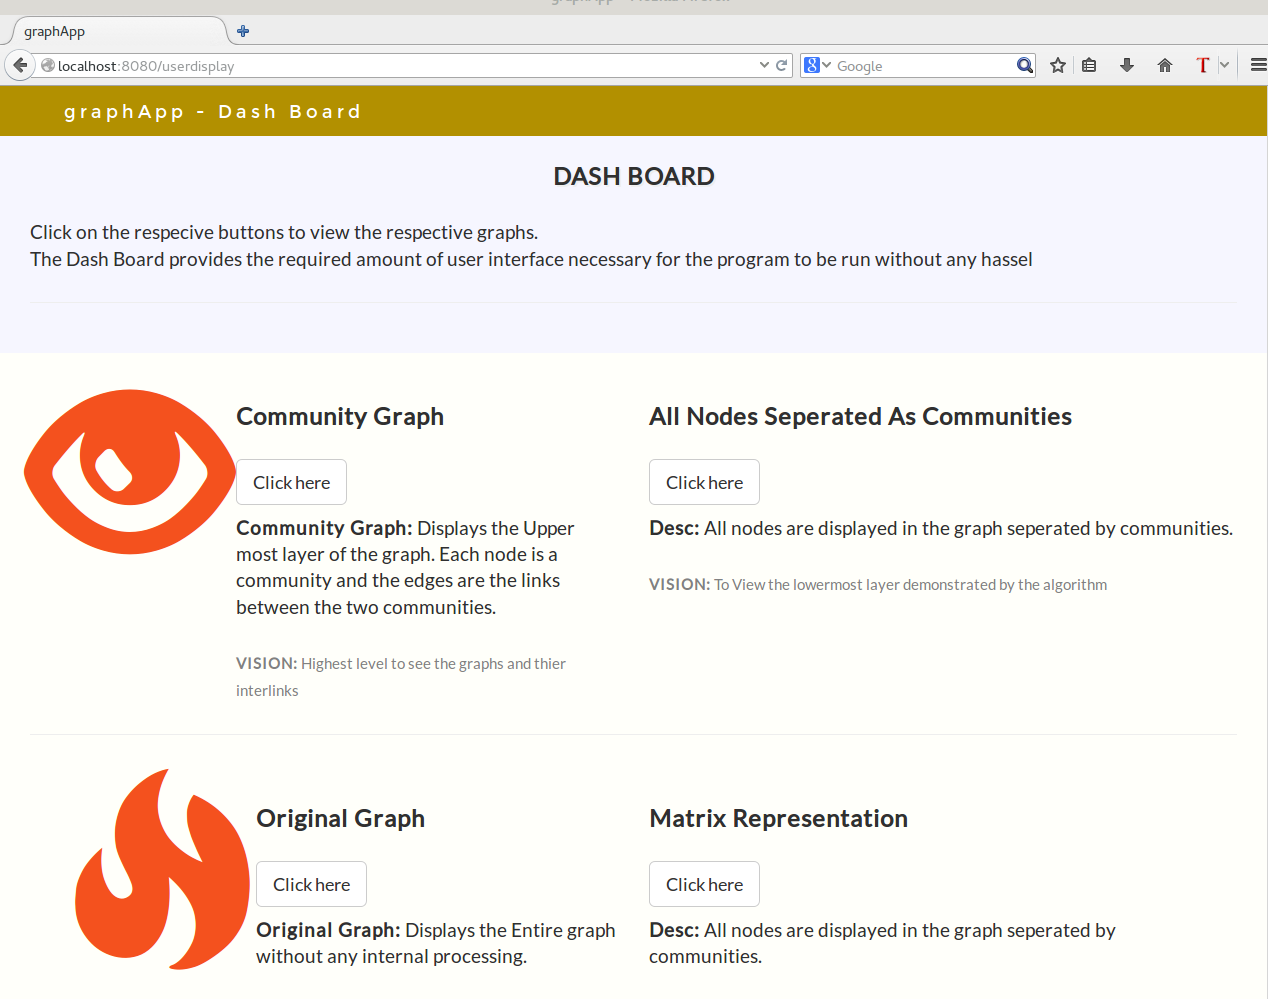
\includegraphics[scale=0.3]{s4.png}
\caption{This Dash board is displayed after the computation process has been completed. }
\end{figure}


\item \textbf{Error Page} In case of mismatch in the format or the password was wrong or the visualization is not possible due the screen size or the browser is not able to handle the large JSON object Errors pages have been genrated to couter act on exceptions. 
\begin{figure}[H]
\centering
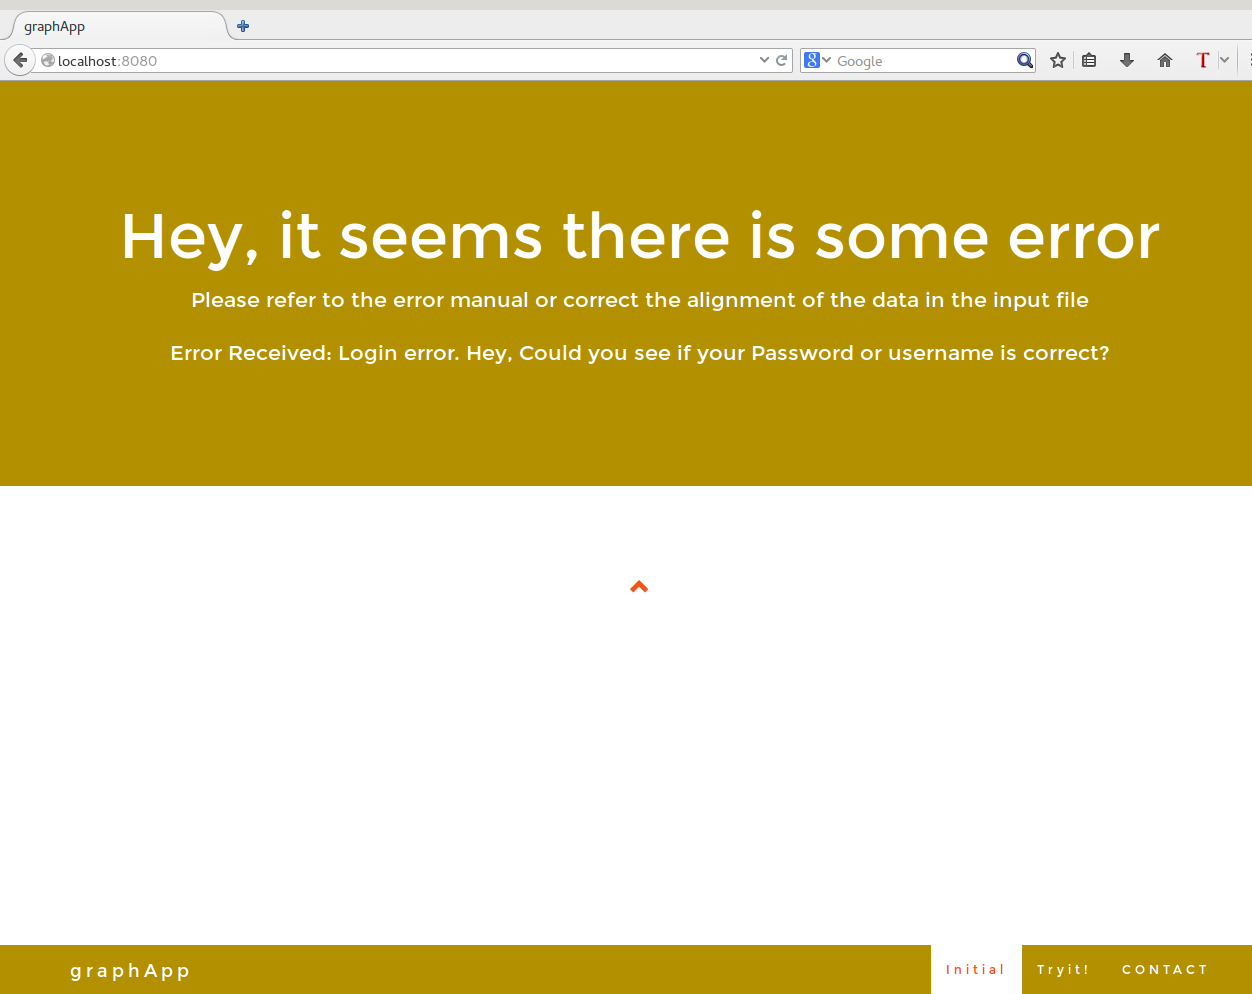
\includegraphics[scale=0.3]{serr.png}
\caption{Error page showing the appropriate error message }
\end{figure}

\end{enumerate}






\section{Implementation Benefits and Drawbacks}
\subsection{Benefits}
\begin{enumerate}
\item The input given can be a weighted or an unweighted graph. The web input is still accepted and the output is generated.
\item Key labels can be assigned to node numbers.  This file if not given the program usses the node number given as id in the input file. 
\item Whether the input is a large graph such as Facebook graph or is a small one such as karate graph the community screen displays the community graph in a size that is propotional with the entire size of the graph on one screen. 
\item Error management involves a seperate class. Hence exact errors can be mentioned and presented to the user in an elegant web interface.
\end{enumerate}
\subsection{Drawback}
\begin{enumerate}
\item Very large graph needs a bigger screen for the entire graph to be displayed.
\item To display such large graphs a browser that could handle large JSON objects is needed along with bigger screen size
\end{enumerate}
\subsubsection{Result}

\chapter{Conclusion and Future Works}
In this section the final conclusion of the project, goals achieved, benefits the project presents to the community and future works are presented. 

\section{Goals Achieved}
In the beginning of the project four major goals were set to be achieved. THe following would enlist in the same order on it s achievement.
\begin{enumerate}
\item In the project we have suveyed a few algorithms that aim in community finding for instance Combo and Louvain keeping in mind that the input is taken from health care domain. 
\item Louvain Community detection algorithm was chosen for community detection and for visualization Alchemy.js and Protovis were selected after considering the input and a few state of the art algorithms. 
\item The algorithms and frameworks thus found were implemented and tests were conducted for finding the effciency of the algorithms.
\item A GUI implementing Web.py and Bootstrap was created combining the visualization and the computation.
\end{enumerate}
Thus, the project succesfully achieved the tasks that were set in the early stages of the project.  
\section{Benefits to the community}
This can be used in places where there is difficulty in visualization of a very complex landscape
of data such as medical domain. In Medical domain a patient can be a vector of diseases and
visualization of such patients (patients graph–which shows relations of how two patients are
similar, a graph in which patient-patient edge weight is the similarity value ) would be useful for
analysing and predicting the disease landscape of a region and in turn multiple regions.
In place of patients if disease/diagnosis graphs can be loaded patterns of occurrence of disease or method of diagnosis can be intuitive from the community that are thus formed. 

\section{Future Works}
In the span of five months we were able to build a basics project by comparing, contrasting, including the one that the directors suggested and choosing the one that is simple and works well. In this project I would like to suggest a few improvements that we would have done given more time. We would like to enumerate on that:

\begin{enumerate}
\item In the Algorihthm part :
\begin{enumerate}
\item The order in which the information is presented can affect the computation of the louvain community detection algorithm. Hence the problem of finding specific heuristics to solve this ordering can improve the louvain algorithm computation time.
\item Another intersting feature is to analyse whether every step in the louvain algorithm gives the exact or nearly exact hierachy of community detection
\item 
The project relies fully on louvain. One can speculate on whether modularity is the only measure that exists. Thinking about a completely new measure would be interesting. 
\end{enumerate}

\item In the visualization Module:
\begin{enumerate}
\item In the current project the communtiy graph is presented seperately from the main graph.  A zoom effect can be introduced to zoom into to community graph to reach different levels of hierachy. 
\item  Double-click on a node to fade out all but its immediate neighbours.
\item We deal with large graphs thus it would be nice to have some search functionalities. jQuery can be used to create an autocompleting search box that can be featured on the graph display page which can search the name of the patient or the treatment that is needed. 
\item Fish eye can be introduced. Since alchemy.js is a framework that runs on d3 it can easily be extended o d3. Hence the fish-eye module can help to view every node along  with it's neighbours in a more expanded format.
\item Developing an editor which is a tool to dynamically add nodes and edges after the graph visualization has taken place. D3 has a ``forced editor" layout and ``Directed forced editor" layout sample which could be useful for further study.
\end{enumerate}
\item In the Overall structure:
\begin{enumerate}
\item The current dash board is before the graph board. The Dash board can be included in the graph board itself to avoid switching back and front in the web application.
\item  A simple Database can be set-up for storing passwords and improvisation on sign-ins can deliver a better personalised user experience. The project provides provision for password input which could be used as a starting point to build on further. 
\end{enumerate}
\end{enumerate}
\section{Availability and requirements}
\begin{enumerate}
\item \textbf{Project Name}: Graph and matrix algorithms for visualizing high dimensional
\item \textbf{Project Homepage}: \url{https://github.com/abhinavsv3/webproject}
\item \textbf{Operating System}: Platform Independent. Preferably Unix--like operating system
\item \textbf{Programming Language}: Python 2.7
\item \textbf{Other Requirements} : Alchemy.js, Python Packages, Web.py
\end{enumerate}

\section{Conclusion}
This is one of the greatest project experience.	
\section{Personal Conclusion}
The project has made my mind very innovative. I can proudly call myself an engineer. My director, prof.Ricard gave me a freedom to think freely and understand the project and made me do the project the way I have analysed it.  This made me develop an new characteristics of learning stuff in the fly and made me feel enthusiastic about working on projects that I have little knowledge on. I am sure given any project I can now make innovation and work hard to bring the project to a better light.

\bibliographystyle{plain}
\bibliography{mybib}{}
\end{document}



